% main.tex, to be used with thesis.tex
% This contains the main work of your thesis.
\nocite{*}

\chapter{Introduction}

This thesis project utilized a dataset of over 2,000 student participants in the Metro College Success Program at San Francisco State University and their control group counterparts to analyze the timing of the students' first non-remedial Mathematics courses, as well as the effect of the extent of progress made by the students through their course sequences on their persistence and graduation outcomes.  

Higher education institutions face ongoing pressure to maximize their retention and graduation rates despite constrained resources.  The graduation rate from the first institution attended by first-time, full-time, bachelor's degree-seeking students at 4-year institutions was 40.6\% nationally for the 2010 starting cohort \cite{NCES_grad}.  Retention of first-time bachelor's degree-seeking undergraduates at degree-granting 4-year institutions has also remained a challenge, with the percentage of first-time undergraduates retained for their second year at 75.3\% nationally for the 2015 starting cohort \cite{NCES_pers}.

The applications of educational data mining and machine learning techniques to student data have proliferated rapidly in recent years as the availability of such data has increased \cite{Romero_2007, Romero_2010, Asif}.  Among many other questions, increasing attention has been devoted to predicting student performance, specifically persistence and graduation outcomes of students based on various demographic and academic factors.  Data mining  \cite{Saa, Shahiri, Asif} and machine learning \cite{Romero_2010, Gopalakrishnan} have been employed to find the strongest predictors of a student's outcome, as well as to help identify intervention methods that have a positive impact on that outcome.  However, the impacts of certain factors that operate at the curriculum level rather than at the student level have been less extensively researched.  Specifically, the impact of the ordered sequence of courses taken by a student on the likelihood of that student to persist and graduate has not been studied in depth \cite{Bhaskaran}.  Furthermore, it has been reported that successful completion of Mathematics courses during the first two years has a significant impact on degree completion, with more than 70\% of students who complete their degree having completed the required Mathematics courses during the first two years \cite{Bhaskaran}.

Institutional efforts to improve retention and graduation have recently been directed at the curriculum level, rather than at the student-specific level.  Learning communities represent one such effort, and have been implemented at many institutions with the objective of improving students' integration into university life \cite{Tinto, Zhao}.  An emerging trend is the evolution of the learning community into the long-duration learning community, which offers academic momentum, integration into university life, and access to timely support services over several semesters at the start of a student's college education \cite{Kolenovic}.  

The challenges of retention and graduation are especially acute for under-represented, under-privileged, and/or first-generation students.  For example, graduation rates for black and Hispanic students from the first institution attended for first-time, full-time, bachelor's degree-seeking students at 4-year institutions was 21.4\% and 31.7\% nationally for the 2010 starting cohort, compared to 45.2\% for white students  \cite{NCES_grad}.  One long-duration learning community program, the Metro College Success Program (``Metro") at San Francisco State University \cite{Metro}, is endeavoring to narrow this gap by concentrating its efforts on these students.  The Metro program groups its participants into different academies based on the student's anticipated major or area of interest (e.g., science, ethnic studies, engineering, among others).  A novel feature of the Metro program is that it incorporates a carefully-designed sequence of scaffolded foundation courses, to be taken during the first two years of college \cite{Metro}.

This thesis project explores the aforementioned curriculum-level factors by taking advantage of a comprehensive dataset consisting of academic and demographic data for over 2,000 student participants in the Metro program for entering cohorts from 2009 through 2016.  This thesis also analyzes a companion dataset that includes the same information for a matched control group of over 2,000 non-participating students.

This thesis applies a multifaceted approach to the dataset.  First, the thesis project examines the timing and performance of Metro students' first non-remedial Mathematics course to elucidate the effect, if any, of the timing of the first non-remedial Math course on performance, persistence, and graduation. The findings revealed a dependence in two aspects: (1) whether a student took one of the STEM-relevant calculus courses or one of the less technical Math courses, and (2) whether this Math course was taken in the first or second year. 

Second, the thesis analyzes the sequences of three scaffolded foundation courses that comprise the foundation of the Metro program's two-year curriculum, and compare the persistence and graduation rates of students who make differing levels of progress through those sequences (i.e., students who complete all three courses, versus two courses, versus only one course).  The findings emphasized the importance of keeping students progressing through their prescribed course sequence.

Third, to generalize the inquiry of the prior section and further elucidate the relationship between sequence progress and persistence/graduation outcomes, the thesis applies sequential pattern mining to identify the sequences of courses taken by the largest number of students in the pool consisting of the Metro program's participants and their control group counterparts.  It then compares the persistence and graduation rates of students who make different levels of progress through those sequences.   Each student's entire academic record is collected and parsed as an ordered sequence of courses, wherein multiple courses taken during a particular semester are treated as a set.  A sequential pattern mining algorithm determined the sequences that were taken by the largest numbers of students.  As such, this approach allowed the academic records of the students themselves, rather than any pre-set notions about what courses the students take, to dictate which course sequences to evaluate.  This aspect of the research consistently revealed the greater importance of the extent of a student's progressing through a sequence, as opposed to the content of the sequence itself.  

Fourth, the thesis applied different classification modeling techniques to assess the relative influence of a student's fifth-term and seventh-term persistence against several demographic and academic factors for predicting graduation status.  The results were consistent with the earlier findings and led to novel insights about the importance of students' curriculum progress relative to other demographic and academic factors such as race, gender, Pell eligibility, and entrance scores.

Overall, this thesis builds on the relatively sparse prior work that utilizes sequential pattern mining to look at sequences of courses to reveal previously-unknown trends.  Particularly, this thesis project contributes novel findings that can inform universities as to how to improve persistence and graduation: by prioritizing strategies and resources that help students continue to make semester-by-semester progress towards their degrees.  Furthermore, this thesis also reveals some of the potential benefits and challenges of sequential pattern mining in analyzing students' course sequence data.

The structure of this thesis is as follows.  Chapter 2 reviews the literature on applications of educational data mining and discusses related work.  Chapter 3 describes the methods used to address each of the questions presented in this thesis.  Chapter 4 presents the major results of the research and some interpretations of the findings.  Chapter 5 discusses the implications of the findings in more detail, including the benefits and limitations of sequential pattern mining, and describes future directions.  Chapter 6 describes the software implementation.  Lastly, Chapter 7 concludes this thesis.

\chapter{Literature Review and Related Work}

Data mining has been applied in a wide variety of ways to improve student outcomes and the quality of educational services.  However, applications of sequential pattern mining with educational data, particularly with course sequences that comprise student curricula, have emerged only recently.  The following sections will examine the state of the literature and the recent scholarship related to this thesis project.

\section{Educational Data Mining in the Literature}

Educational data mining (EDM) has proliferated rapidly in recent years \cite{Pena,Romero_2007}.  The users of EDM applications include learners, educators, course developers, institutions, and administrators.  Table \ref{table_Romero} summarizes some of the educational tasks for which EDM has been applied, and lists some of the techniques that have been applied to each task type \cite{Romero_2010}.  It should be noted that the Table does not do justice to the tremendous variety of techniques that have been used in tackling EDM problems, and as such it should not be interpreted as an exhaustive treatment of the subject.   

\begin{table}[htbp]
\begin{center}
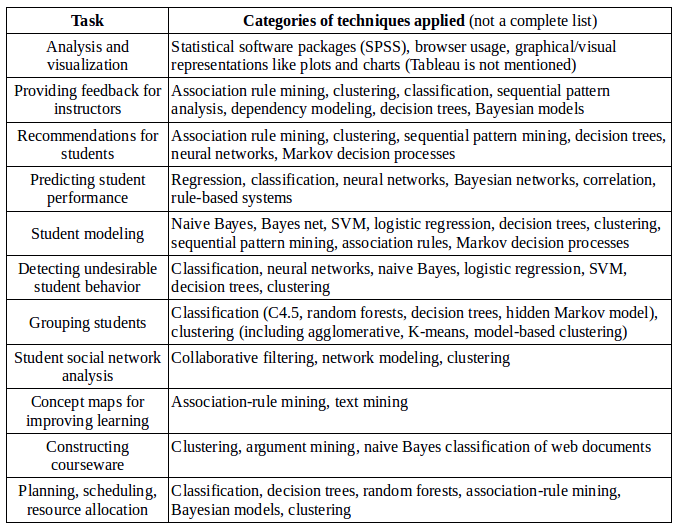
\includegraphics[width=\textwidth]{root/tables/RomeroSurvey.png}
\end{center}
\caption{Tasks and techniques in educational data mining.}
\label{table_Romero}
\end{table}

In a comprehensive meta-analysis, Romero and Ventura \cite{Romero_2010} provide an excellent introductory look at EDM and its applications.  The authors describe the numerous unanswered questions and areas where EDM can improve and grow.  The authors give very brief descriptions of over two hundred papers in this survey, broken down both by data types, by tasks, and by data mining techniques used.  It is clear that EDM, despite being in its adolescence according to the authors, has seen a great many publications and applications as of 2010.  As such, this paper provides a very useful high-level view of the EDM landscape.

A more recent meta-analysis of EDM research \cite{Pena} provides some insights on the current trends and future applications of EDM for improving education.  The modeling of student behavior and performance has experienced tremendous growth in the last few years, as researchers strive to identify criteria that place certain students at risk of poor class performance (e.g., reduced attendance or a failing grade) \cite[Sections 3.1-3.2]{Pena}.  Likewise, scholarship of the best algorithms and modeling techniques has increase rapidly since 2010 \cite[Section 4]{Pena}.  Thus, the ongoing proliferation of EDM studies include work both to improve education and to improve the tools and approaches to analysis that are employed by EDM scholars. 

As described in more detail in the following paragraphs, a subset of the broad landscape of EDM research described in \cite{Romero_2010} and \cite{Pena} involves prediction of student performance and long-term outcomes, such as persistence and graduation.  Many of the features considered in generating predictive models include demographic and personal factors, such as age, race, gender, and family educational history (e.g., highest education level attained by the mother and father of a student) \cite{Shahiri}.  Another category of student features relates to the activities of the student, such as whether and how much students participate in extracurricular activities and the extent of their social networks.  Additional factors such as student interests, study behavior, and family support have been included in some analyses \cite[Section 3.1]{Shahiri}.  Lastly, student performance in their courses, as measured by either cumulative GPA or the grade points earned in particular courses, is another frequently-used factor in predicting long-term student outcomes. 

The work reported by Asif \cite{Asif} exemplifies the use of EDM to improve a curriculum through the use of student performance data.  The problems addressed in the work were to identify courses as indicators of a student's overall, curriculum-long performance, and to identify progressions of student performance up to and including the indicator course, in an effort to best understand student outcomes.  The study analyzed the performance of students seeking a four-year degree in the Information Technology major of a Pakistani university.  The available dataset included the grades of 210 Information Technology-majoring students in the 2007-2008 and 2008-2009 entering cohorts in a few selected courses (specifically, five required courses) taken by those students \cite[Table 1]{Asif}.  Thus, performance in each of those courses by a student comprised the input feature set for that student.  The response variable was coded as a single value, computed as 10\% of the first-year average examination mark, 20\% of the second-year average mark, 30\% of the third-year average mark, and 40\% of the fourth-year average mark.  This value was then transformed into an ordinal categorical variable with five levels.  One disadvantage of the dataset was its unbalanced nature: only one student in the entire dataset achieved the highest category out of the five ordinal categories of the response variable; over 80\% of the students in the dataset had the second or third out of five response variable values (i.e., over 80\% of the students in the dataset were in level two or level three out of five levels of the response variable).  

Naive Bayes, random forest, neural network, and 1-nearest neighbors classifiers were used to predict the aforementioned response variable for each student, with naive Bayes representing the most accurate model.  The random forest model revealed evidence that low performance in Applied Physics in the first year, or in Logic Design in the second year, were the courses most strongly predictive of poor long-term performance.  However, the paper did not report any feature elimination strategies for any of the models, which would have been useful for determining which features were most important in reaching the highest classification accuracy scores reported.  

More recently, Saa \cite{Saa} investigated the problem of determining the effect of social and personal factors of students, as well as the effect of their academic performance in a certain semester, on the student's performance in the following semester.  As such, the study sought to develop predictive models for student performance in the short-term, i.e., the next semester.  The dataset consisted of voluntary surveys completed by 270 students, across different departments of a four-year university in the United Arab Emirates.  The survey gathered information about demographic (gender, race, national origin, living location, commute length and transport mode), economic (financial aid, family income) and personal (language spoken, family size, parents' marital status and careers) factors, and combined these with the student's high school GPA and the GPA in the semester prior to taking the survey (\cite[Table 1]{Saa}).  All  of these factors were coded as categorical variables and used as input features for decision trees that employed different feature importance algorithms: C4.5, CART, CHAID, and ID3.  No hyper-parameter tuning was reported for any of the models, which were then compared with a naive Bayes classification model. For the response variable (GPA in the next semester), four ordinal categorical values were created and used (Excellent, Very Good, Good, Pass) as the output classes. 

The classification models achieved accuracy between 33\% and 40\%, with the CART implementation of the decision tree model yielding the highest accuracy.  However, the work does not report any feature elimination strategies or any attempt to identify the most important features used by the models.  The authors interpreted the conditional probability distribution matrix \cite[Table 5]{Saa} as indicating that gender, high school grades, mother's occupation status in a service profession, and whether a student is a scholarship recipient are the factors with the highest prior probability for those students with very good or excellent grades in the next semester (the response variable).  The authors did not share any insight as to how these findings can lead to an improved curriculum, or how they should inform whether and when the university conducts interventions with certain students.  Moreover, it would have been interesting to see the results of feature selection or elimination efforts, so as to determine whether the accuracy improved by leaving out features with minimal or no importance to the classifications.  

The next section focuses on a technique, sequential pattern mining, that has emerged relatively recently in the EDM landscape but is seeing increasing use.   

\section{Applications of Sequential Pattern Mining}
\label{section_spm}

Sequential pattern mining is well-suited for addressing questions wherein the data can be characterized as an ordered collection of events or actions \cite{Agrawal}.   In the majority of applications of sequential pattern mining for educational data, the actions under study involve learning behavior, such as when students participate in discussion forums or view class materials \cite{Jiang, Chen} or when students perform various actions in collaborative problem-solving environments \cite{Martinez, Munk, Perera}.  The next few paragraphs describe examples of these applications in more detail.  

As an interesting example of the use of sequential pattern mining to understand learner behavior, Martinez \cite{Martinez} tackled the problem of determining frequent patterns in the actions of primary-school learners in collaborative settings.  The dataset included the log traces of a problem-solving tabletop application for use by elementary school students between the ages of eleven and fourteen.  The tabletop application presented each of the six groups of three students each with a question on any subject (e.g., math, history or physics) and the information necessary to solve the question.  The tabletop application's log trace recorded all of the transactions between the students and the system.  The dataset collected over 17,000 distinct actions performed by the six groups of students over twelve different logged sessions.  There were seven distinct possible actions: (1) move; (2) enlarge; (3) reduce to normal size; (4) shrink; (5) add to a group; (6) remove from a group; and (7) combine contents of two screens into one, so that both are visible at the same time.  Each of these actions was performed on digital screens that contained specific contents identified by a unique label; hence a certain action was a tuple consisting of (student-identifier, action, content-identifier, time-of-action).  Within each session, these actions took place in an ordered sequence, making them amenable to sequential pattern mining.  Students were categorized into high-achieving and low-achieving groups based on their success in solving the questions.  

Using the foregoing dataset, the authors used sequential pattern mining to find the most frequent sequential patterns of actions.  The authors also associated those sequential patterns with the students' achievement level.   The results of clustering revealed interesting insights about the sequences of steps undertaken by more successful students and by less successful students \cite[Table 1]{Martinez}.  For example, the students who performed fewer of the ``combine" actions (i.e., students who combined multiple information screens with less frequency) performed better than students who performed many ``combine" actions.  The authors interpreted this finding as suggesting that students who let their attention be drawn to too much information at a time have greater difficulty in solving the problem.  Thus, this study provided greater transparency to the learning process of the student participants and revealed interesting insights about how groups of students solve problems.  

Perera \cite{Perera} utilized a similar problem-solving approach with university seniors in a software engineering course.  The authors addressed the problem of identifying which actions and resources in the software development process contributed most to the students' successful realization of the course goal: to build an effective software application by the end of the course.  More specifically, the students, working in groups of five to seven, were tasked with developing a software application for a client.  The students were required to use a development tracking system that included the SVN version control system, a ticketing system, and a group wiki for shared web pages \cite[Section 3.2]{Perera}. The available dataset thus consisted of all events in the activity log of the tracking system.  Those events included: commits to the SVN repository; the creation, modification, or removal of the wiki pages; and the creation and resolution of bug tickets.  The dataset included between 1,400 and 2,500 distinct tracked events for each of seven student groups.  Lastly, the authors categorized each group as successful or unsuccessful.

Using the foregoing dataset, the authors performed clustering and sequential pattern mining.  In the clustering phase, the authors determined that the most successful groups made the most extensive use of the wiki pages while resolving tickets.  The authors subsequently incorporated this finding into future teaching of the course.  For sequential pattern mining, the authors used a modified form of the a priori algorithm for frequent item sets \cite[Section 6.1]{Perera}.  The authors translated the raw sequence data from the tracking system into sequences of character strings usable by the Weka data mining tool \cite[Table 9]{Perera}.  By associating frequent sequential patterns with the course outcomes of the groups who performed those patterns,  the authors found that the best-performing groups had the highest frequency of alternating SVN-wiki events (in other words, these groups had the highest frequency of accessing the wiki pages before and after making commits to the SVN repository).  Meanwhile, the lowest-performing groups had a high frequency of wiki access but a low frequency of SVN commits.  The authors concluded that for the low-performing groups, the students' efforts at understanding the wiki pages were not being used to support software development.  Thus, through the use of sequential pattern mining, the authors gained actionable insights into how to better teach the course and how to better advise students on the best ways to complete their development projects.

Massive online open courses (MOOC) have represented another context for sequential pattern mining research, since the learning actions of the student participants in those courses are saved in activity logs.  The study reported by Jiang \cite{Jiang} is illustrative.  The problem that the authors address is to create a way to better manage forum contents by matching video clips viewed at certain times with forum threads whose contents are edited at similar times.  Thus, this work investigates the association between forum threads and subtitles of video clips that are available as learning resources to the students.  The available dataset included the subtitles of video clips, discussion forum contents, and learners' click-stream logs associated with a Coursera course and a course of China University (a leading MOOC platform in China).  The courses had over 3,000 and over 10,000 student participants respectively.  The authors indicate that only a limited set of labeled data was available, and therefore they consider the work an unsupervised learning exercise and do not seek to generate any classification or regression models.  The labeled data was used to evaluate several different approaches for clustering related forum contents together based on the video clips and click-stream events.  The authors' proposed approach utilizes the idea that the order of click-stream events associated with the learners' viewing of videos, reading threads, or posting threads can reflect document-level latent similarity \cite[Figure 1]{Jiang}.  
The authors reveal that for the Coursera course, their proposed approach yielded higher P@1, P@3, and P@5 precision scores than bag-of-words, Word2Vec, or Para2Vec models against which their approach was compared.  (Recall and F1 scores were not reported.)  For the larger dataset (10,000 students), their approach offered lower precision than the other models at P@3, and P@5.  Overall, this work suggests the potential utility of sequential pattern mining as another option for revealing insights from the activities of learners.

The next section will more closely examine the relatively sparse literature specific to the applications of sequential pattern mining to academic curricular data.  

\section{Related Work}

Previous works have employed sequential pattern mining in analyzing educational data in various contexts.  As explained in more detail in the preceding chapter, a growing body of work has applied sequential pattern mining to the activities of learners in massive online open courses (MOOC) \cite{Jiang} as well as to how groups of students at the elementary school \cite{Martinez} and university \cite{Perera} levels collaborate to solve problems and complete complex projects.  These studies demonstrated that sequential pattern mining can lend transparency to the learning process by uncovering the frequent patterns in which learning actions occur, and those patterns can then treated as features when analyzing how successful the students were in completing their tasks.

However, the application of sequential pattern mining to sequences of \textit{courses} taken by students during their academic careers is still very much an emerging research direction.  Campagni \cite{Campagni} applied sequential pattern mining to address the problem of how the timing of computer science students' completion of course examinations affected students' graduation outcomes.  In the higher education institution under study, students were allowed to take the examination in a different semester from which the course is taken, so that the order of examinations is not necessarily the same as the order of courses.  

The dataset consisted of the courses taken by 141 graduate students in the Computer Science department of an Italian university.  Each student's academic career was thus represented as a sequence of examinations ordered by semester, and examinations taken during the same semester comprised an non-ordered set.  For example, a student's academic career might be represented by the ordered sequence of examinations \textless\{2,3,7\} $\rightarrow$ \{1,4\} $\rightarrow$ \{5,6\}\textgreater{}.  This sequence represents that the student took the examinations for courses 2, 3 and 7 in semester 1; examinations for courses 1 and 4 in the second semester; and examinations for courses 5 and 6 in the third semester \cite[Section 3]{Campagni}.  This work assumed the existence of an ideal sequence, in which each student takes the examination at the end of the semester in which the associated course was taken.  The study used sequential pattern mining to generate each student's sequence, and to compute each student's deviation from the ideal sequence using bubble sort distance.  

Using this approach, the study revealed that greater deviation from the ideal sequence of examinations (i.e., taking more examinations in semesters other than the ones in which the corresponding courses were taken) led to decreasing likelihood of graduation.  The authors also used the sequential patterns to generate new features.  For example, students who took the examinations for courses 1 and 5 at the same time were given a positive value for a new feature reflecting that those students exhibited the \{1, 5\} sequential pattern \cite[Table 8]{Campagni}.  The authors used these features to identify particular examinations that the students delayed taking the longest, leading to the largest separation in time between the underlying course and the examination.  These findings provided insights for the authors for advising students not to delay the examination in that particular course.

As exemplified in \cite{Campagni}, sequential pattern mining offers the ability not only to extract sequential patterns from course sequences, but also to generate new features that can be added to existing feature sets to provide a new dimension to the analysis of student data for predicting persistence and graduation.  Recently, Gopalakrishnan \cite{Gopalakrishnan} addressed the problem of identifying useful features for the prediction of fifth-term persistence, seventh-term persistence, and graduation for the student participants in a long-duration learning community program, the Metro College Success Program (``Metro") at San Francisco State University \cite{Metro}.  The Metro program, while open to any incoming first-time, full-time freshmen, targets students from under-represented minorities and disadvantaged socioeconomic and personal backgrounds, as reflected by Pell eligibility and first-generation  student status.  Students of color exhibit lower persistence \cite{NCES_pers} and graduation \cite{NCES_grad} rates.  Metro's mission is to bolster these rates by providing enhanced services to these students during their first two years of college.  The enhanced services include: reminders and support during course registrations; academic advising; access to a tutoring center; and frequent coordinating and counseling interactions.  Metro also emphasizes learning communities, to instill a sense of belonging among students \cite{Tinto, Chen}.   

The dataset in \cite{Gopalakrishnan, Gopalakrishnan_thesis} consisted of twelve different features for 651 students in 2009-2013 entering cohorts of the Metro program.  The available features included Pell eligibility; first-generation status; EOP status; ELM and EPT entrance scores; household income; education level of each parent; race; start term; department; and gender, among others.  The study applied different feature selection algorithms to the dataset to identify those features most strongly predictive of the third-term, fifth-term, and seventh-term persistence and graduation outcomes of the students \cite[Table 3]{Gopalakrishnan}.  ELM score or the mother's education level were found to be the most important features for predicting graduation by six out of the seven feature selection algorithms.  This work also developed and tested classification models based on Adaboost, extra trees, K-nearest neighbors, linear SVC, and naive Bayes classifiers \cite{Gopalakrishnan_thesis}.  The study revealed the difficulty of predicting graduation based solely on personal and demographic factors: the algorithm that achieved the highest accuracy was naive Bayes, with an accuracy score of roughly 66\% \cite[Figure 16, top]{Gopalakrishnan_thesis}.  The algorithm with the lowest classification accuracy was extra trees, with an accuracy of 54\%.  

Overall, these findings demonstrated that a student's university career is a complicated phenomenon, and the student's long-term outcome is not easily predicted based on demographic or personal factors about a student. Consequently, this work seeks to leverage sequential pattern mining in order to find curriculum-level factors (i.e., factors that operate over multiple-semester course sequences) that can be added to the personal and demographic student attributes studied in \cite{Gopalakrishnan} to yield not only improved classification models for predicting persistence and graduation, but also new insights about the importance of multiple-semester course sequences and how they affect a student's long-term outcome. 

This thesis extends the aforementioned applications of sequential pattern mining to the courses taken across multiple semesters by the students at San Francisco State University to determine whether the most commonly-observed sequences offer better persistence or graduation for the students who take those sequences.  This thesis also extends the study of Gopalakrishnan \cite{Gopalakrishnan} by making use of a larger student dataset that now includes the years up to and including 2016 as well, and as such, this thesis covers many more students over a longer period.  Furthermore, this thesis considers features that capture the extent by which students progress through their chosen course sequences, extracted using sequential pattern mining techniques as described next.

\chapter{Methods}

This section describes the problem-solving methodologies that were employed to address the aforementioned four problems, which are:

\begin{enumerate}
  \item The timing of students' completion of certain Math courses, and its effect on persistence and graduation.
  \item The effect of increased progress through the Metro program's sequence of three foundation courses on persistence and graduation.
  \item The extraction of the most frequently-taken course sequences and the effect of increased progress through those sequences on persistence and graduation.
  \item Determination of the relative importance of sequence progress as a feature, compared to demographic and personal features, in predicting graduation outcomes.
\end{enumerate}


Figure \ref{modules} depicts the software modules used to address these problems, each of which is discussed in turn in the remainder of this section.

\begin{figure*}[htbp]
\centering
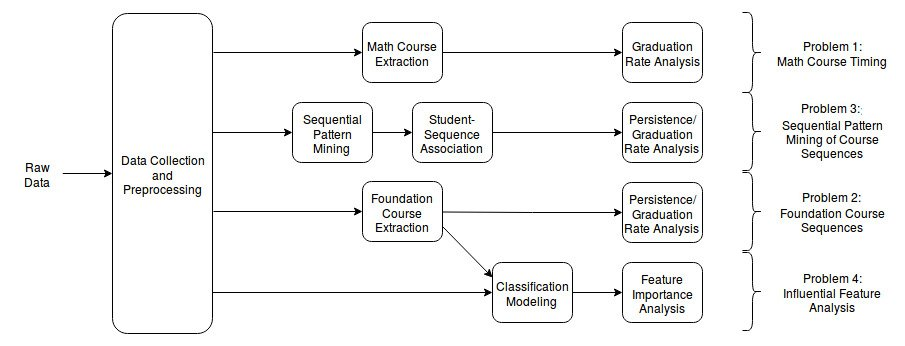
\includegraphics[width=\textwidth]{figures/modules.jpg}
\caption{Major functional modules associated with each problem addressed in this thesis.}
\label{modules}
\end{figure*}

\section{Data Collection and Preprocessing}

First, the relevant data were collected from the Metro program and from the university's student records and institutional research departments.  The general characteristics and features of the dataset are shown in Table \ref{table:students} and broken down by student categories: the participants of the Metro program; the control group of comparison students; and all other students who started at the university as first-time, full-time freshmen and for whom complete records of the indicated features were available.  Students in the control group were matched with program participants based on first-generation status, under-represented minority (URM) status, gender, Pell eligibility and needing remediation in Math and/or English.  For each category, the cohorts include the entering classes from 2009 through 2016.  In the preprocessing phase, each student's complete record of features as shown in Table \ref{table:students} was checked to ensure that each student had at least one semester of course registrations and grades.  In each student's record, the semesters were numbered such that the student's first semester as an entering freshman was semester 1, and so on.  Semesters in which a student did not register for classes were still assigned the next number.  Student records that did not have third-, fifth-, and seventh-term persistence and graduation status were removed, because we did not impute missing values for these response variables.  Otherwise, missing values were left in place but omitted for statistical calculations.  Table \ref{table:students} indicates the size of the resulting dataset. 

The data collection and preprocessing steps were implemented using the Python programming language (v. 2.7.12) and the Pandas data manipulation and analysis library \cite{Pandas}.  Additional implementation details are provided in Chapter \ref{chapter_implementation}.       

\begin{table}[htbp]
\centering
\caption{Characteristics of the student dataset.}
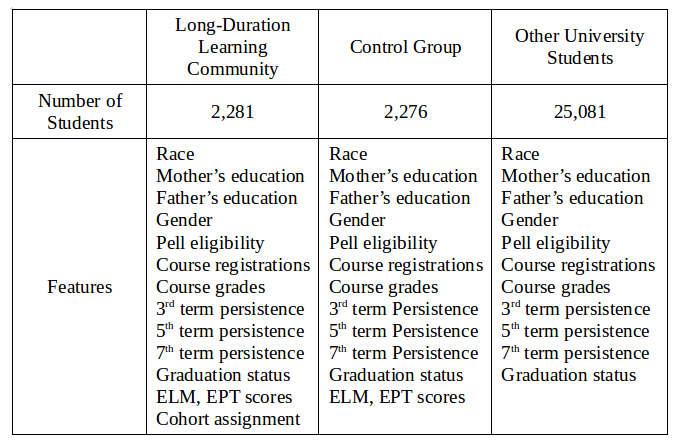
\includegraphics[width=0.75\textwidth]{tables/student_data_sets.png}
\label{table:students}
\end{table}

\section{Math Course Analysis}

The Metro program assigns its students to different academies.  Each academy is a ``school within a school" that provides its students with a variety of services, such as assistance with and reminders about course registration, tutoring, academic advising, and academic planning \cite{Metro}.  Each academy also provides a pathway of recommended courses (some of which are required, as described in the next section). Each academy's pathway of courses includes a recommended Mathematics course.  Some of the Mathematics courses are precalculus or calculus courses oriented towards students interested in or majoring in STEM subjects, while other courses are less technical and geared towards non-STEM areas (Table \ref{table:math_courses}).  For brevity, the calculus-related courses will be referred to as ``STEM" and the other courses as ``non-STEM".  

Using the set of student records described in the preceding subsection, the semester number in which each student in the Metro program and the associated control group took the recommended Math course was extracted (Figure \ref{modules}, Problem 1).  Also extracted were the student's grade in that course and fifth-term persistence, seventh-term persistence, and graduation outcome.  We then evaluated the performance of the students in each of the Math courses in Table \ref{table:math_courses}.  We also determined the persistence and graduation rates of students, broken down by whether they took a STEM or non-STEM Math course and whether they took that course in the first year (semesters 1 or 2) or second year (semesters 3 or 4).  For this question we again considered the combined pool of student participants in the Metro program and their control group counterparts.  The Chi-square statistical test was used to validate whether there is a relationship between the year in which the student took the Math course and fifth-term persistence, seventh-term persistence, and graduation status for both the STEM and non-STEM courses.  The Scipy statistical computing library for Python \cite{Scipy} carried out this task.  Additional implementation details are provided in Chapter \ref{chapter_implementation}.

Note that throughout this thesis project, the 2009-2015 cohorts were considered when determining fifth-term persistence, 2009-2014 cohorts for seventh-term persistence, and 2009-2013 cohorts for graduation status.

\begin{table}[htbp]
\centering
\caption{Math courses studied in this thesis.}
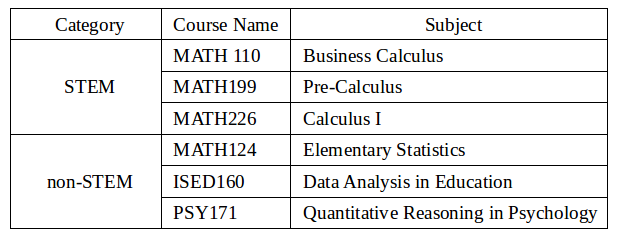
\includegraphics[width=0.75\textwidth]{tables/Table_math.png}
\label{table:math_courses}
\end{table}

\section{Foundation Course Sequences}

As described in the Introduction, the Metro program requires each student to enroll in an academy-specific sequence of three carefully-designed and scaffolded foundation courses that emphasize community-building and social justice.   The Metro program consists of multiple academies, and each participant in the program is assigned to one of the academies based on that student's cohort.  For example, a student starting in 2014 may be a participant of the ``2014 Health Studies" cohort, and as such is assigned to the Health Studies academy.  Each academy's three-course sequence may include different courses, tailored to that academy.  A summary of the three-course sequence and when each course is taken is shown in Figure \ref{capstone}.  Program participants are required to take all three courses, and the student's completion of the Metro program is contemporaneous with completion of the capstone course. 

\vspace{5mm}
\begin{figure}[htbp]
\centering
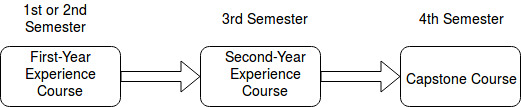
\includegraphics[width=0.75\textwidth]{figures/capstone.jpg}
\caption{Foundation course sequence of the Metro program.}
\label{capstone}
\end{figure}
\vspace{5mm}

As such, the Metro program afforded an opportunity to analyze the effect of increased progress through each student's prescribed three-course sequence on fifth-term and seventh-term persistence and graduation. 

Let $S$ represent the set of students in the Metro program, and $F$ = \textless $f_1 \rightarrow f_2 \rightarrow f_3$\textgreater{} represents the sequence of three foundation courses for a particular student $s_j$.  The pseudo-code for analyzing their progress through $F$ is depicted in Figure \ref{pseudo_foundation}.     

\begin{figure}[htbp]
\centering
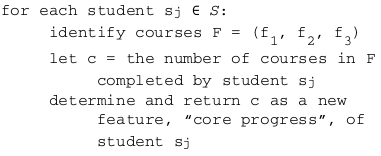
\includegraphics[width=0.6\textwidth]{figures/pathwayprogress.png}
\caption{Pseudo-code for foundation course sequence analysis.}
\label{pseudo_foundation}
\end{figure}

Each student's extent of progress through the three-course sequence of that student's academy is determined based on the number of courses that the student passed.  As indicated by the downward-angled arrow in Figure \ref{modules}, that number of courses becomes a new feature (referred to hereafter as ``core progress") for that student and is considered in the feature ranking problem described in Section \ref{feature_importance_subsection}.  Students were aggregated across all academies by their core progress values and computed the percentage of students at each core progress value (i.e., 1, 2, or 3) with positive fifth-term and seventh-term persistence and graduation outcomes.


\section{Sequential Pattern Mining}
\label{methods_section_spm}

A brief description of the concept of sequential pattern mining is presented next; for interested readers, Pei \cite{Pei} presents a more comprehensive treatment of the subject and of the PrefixSpan algorithm employed in this thesis.

Let S = \{$s_1$, $s_2$, ... $s_N$\} be the collection of N student records, wherein each student record $s_i$ consists of the entire undergraduate academic career of student $i$.  Specifically, each record $s_i$ consists of an ordered collection of semesters, each of which in turn consists of the non-ordered set of $k_j$ course(s) $c_1$, $c_2$, ... $c_{k_j}$  taken in semester $j$: 

$s_i$ = \textless\{$c_1$, $c_2$ ... $c_{k_1}$\}  $\rightarrow$ \{$c_1$, $c_2$ ... $c_{k_2}$\} ...\textgreater  

Moreover, semesters in which no courses were taken are represented as an empty set, as in the following example in which a student took no courses in the second semester:

$s_i$ = \textless\{$c_1$, $c_2$ ... $c_{k_1}$\} $\rightarrow$ \{\} $\rightarrow$ \{$c_1$, $c_2$ ... $c_{k_3}$\} ...\textgreater

Let the minimum support m$_{sup}$ represent the proportion of N student records that contain a given sub-sequence.  Sequential pattern mining algorithms extract all sub-sequences that occur in at least N*m$_{sup}$ of the student records.  In a simple three-student example, consider the following set of student records:

Student 1: \textless\{MATH100, ENG30\} $\rightarrow$ \{MATH101, ENG35\} $\rightarrow$ \{MATH102\}\textgreater

Student 2: \textless\{MATH100, PHIL50\} $\rightarrow$\{PHYS140\}\textgreater

Student 3: \textless\{MATH100\} $\rightarrow$ \{MATH102\}\textgreater

If m$_{sup}=0.5$, then the sub-sequence \textless MATH100  $\rightarrow$ MATH102\textgreater{} would be the only sequential pattern of length 2 returned.  The patterns \textless MATH100\textgreater{} and \textless MATH102\textgreater{}, each of length 1, would also be returned.  The elements in the sub-sequence are not required to be in adjacent sets.  Hence, in the above example, \textless MATH100  $\rightarrow$ MATH102\textgreater{} is a valid sequential pattern even though the pattern spans three semesters for Student 1 rather than two semesters for Student 3.  Thus, in this thesis, given the set of student records and a certain m$_{sup}$ threshold, a sequential pattern mining algorithm identifies the complete set of sequential patterns in the collection of student records.  

Given a  set $S$ of the course registrations per semester for all students, m$_{sup}$ threshold, and minimum length l$_{min}$, then the pseudo-code associated with mining and processing the sequential patterns from the collection of student records in this thesis project is shown in Figure \ref{pseudocode}. 

\begin{figure}[htbp]
\centering
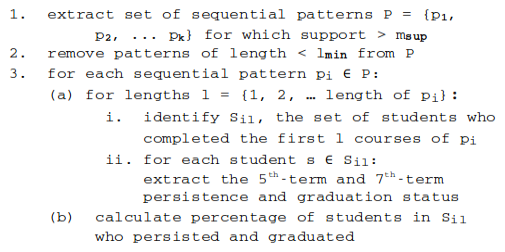
\includegraphics[width=0.9\textwidth]{figures/pseudocode_spm.png}
\caption{Pseudo-code of sequential pattern mining.}
\label{pseudocode}
\end{figure}

As depicted in Figure \ref{pseudocode}, all sequential patterns whose support exceeds m$_{sup}$ and whose length exceeds the specified minimum length $l_{min}$ were extracted from the complete set of student records in step 1. This step yields a set P of qualifying sequential patterns.  In the second step, each qualifying sequential pattern is used as a reference pattern, and the students whose academic records contained this reference pattern are identified and returned.  The step identified the ten most frequently-encountered sequential patterns of three courses; in other words, the step identified the ten length-3 patterns that were taken by the largest number of students in the dataset.  In step 3, students whose records contained a contiguous subset of each of those ten sequential pattern were identified.  For instance, if a reference pattern includes the courses \textless MATH100 $\rightarrow$ MATH101 $\rightarrow$ MATH102\textgreater{}, then we identified not only students who took that entire pattern, but also students who took only the first n$<$3 of those courses.  For example, a student whose record only includes \textless MATH100 $\rightarrow$ MATH101\textgreater{} would be identified when examining how many students took only two of the three courses in that reference pattern.  Identifying these students enabled the comparison of the effects on graduation of partial completion of frequently-encountered course patterns.

To examine the effect of increased progress through sequences, the top ten most frequent sequences of length 3, and the top five most frequent sequences of length 5, were further analyzed as depicted by Figure \ref{pseudocode}.  For every student in the pool consisting of the Metro program and their control counterparts, we determined how many of the courses in each sequence in the top ten (for length 3) and the top five (for length 5) were passed by that student, wherein a passing result is achieved by any grade including or above a C- grade.  For example, if a length-3 sequence includes courses \textless MATH110 $\rightarrow$ MATH120 $\rightarrow$ MATH130\textgreater{} and a certain student passed MATH110 and MATH120, that student is given a progress indicator of 2 for that sequence.  We then determined the persistence and graduation rates of the collection of students for each progress indicator value.  Lastly, we aggregated the collections for each of the top ten length-3 sequences and computed the percentage of students at each progress level with positive fifth-term and seventh-term persistence and graduation outcomes.  Likewise, for the top five length-5 sequences, the possible progress indicator values are 1 through 5.  We aggregated the collections for each of the top five length-5 sequences and determined the seventh-term persistence and graduation rates as a function of progress level.

The following example demonstrates the aggregation.  A hypothetical university has a pool of four students: Student A, B, C, and D.  Students A and B passed MATH110 and MATH120 but never passed MATH130.  Students A and B therefore completed 2 of the courses in this sequence, and have a progress value of 2.  Meanwhile, Students C and D passed all three courses, so each student has a progress value of 3.  Now, assume that student B never graduated, but students A, C, and D did graduate.  In that case, for the two students (C and D) with a progress value of 3, 100\% of them graduated, so the progress level ``3 courses" would have a 100\% graduation rate.  Meanwhile, the ``2 courses" bar would have a 50\% graduation rate, since only 1 of the 2 students with that progress level graduated.

To accomplish the aggregation, for each of the top ten 3-length sequential patterns, the aforementioned process was conducted to count the numbers of students at each progress level.  To afford an aggregated view of these data, the counts of each progress level (1, 2 and 3) were each added together.  For example, if sequence 1 had 20, 30, and 40 students with progress values 1, 2, and 3 respectively, and sequence 2 had 52, 63, and 74 students with those progress values, then the aggregated totals would be 72 (52 + 20) for progress value 1, 93 (30 + 63) for progress value 2, and 114 (40 + 74) for progress value 3.  

The sequential pattern mining task was carried out using the Sequential Pattern Mining Framework (SPMF), a Java-implemented library of data mining algorithms \cite{Viger}.  Of the available pattern mining algorithms in SPMF, the PrefixSpan algorithm was chosen because of its efficient performance as reported in other studies \cite{Pei, Maylawati} and because it accepted string sequences \cite{Viger_PrefixSpan}.  Python programming was used to identify the students whose records included the sequential patterns.  A more detailed description of the implementation is provided in Chapter \ref{chapter_implementation}.



\section{Classification Models and Feature Importance}
\label{feature_importance_subsection}


While the tasks of the prior two sections analyzed the extent of a student's progress through course sequences, this task weighs the relative importance of that progress against other features, such as race, gender, Pell eligibility, and ELM and EPT entrance scores.  To carry out this task, classification models were developed and trained using the features identified in Table \ref{table:students} for each of the associated pools of students indicated in the Table.  (Note that, in order to maintain a focus on curriculum-level features rather than specific courses and to avoid making comparisons between cohort years, the following features were not considered for this task: individual course registrations or grades; or cohort.)  To assess classification accuracy, we compared naive Bayes, logistic regression, and random forest classification models using the long-duration learning community students and their control group counterparts in a combined pool.  Naive Bayes is a well-established and relatively simple probabilistic modeling technique that has demonstrated strong results despite its assumption of the independence of its features in making predictions of output classes \cite{Rish}.  Given a student with a certain set of input feature values, logistic regression models the probability that the student belongs to a given output class, and has been widely used in EDM \cite{Hastie, Romero_2010}.  Random forest classifiers use decision trees as building blocks, and a random selection of the input features is used to split each node to grow each tree \cite{Breiman}.  Moreover, the random forest algorithm can generate rankings of the influence of each input feature on the accuracy of the predictions, yielding the relative importance of each feature \cite{Hastie, Louppe}.  Random forests have also enjoyed a great deal of popularity in EDM applications \cite{Shahiri}.  

To assess the relative importance of fifth- and seventh-term persistence compared to personal factors, such as race, gender, and entrance scores, the accuracy of each of the aforementioned models was assessed using ten-fold cross-validation for each model type.  Recursive feature elimination \cite{Genuer} in conjunction with the random forest classifier was used to identify the subset of features that gives rise to the best model.  The steps of this algorithm are as follows:
\begin{enumerate}
  \item Determine the importance of each feature for the full classification model, which uses all available input features.  
  \item Eliminate the feature that had the lowest Gini importance, and build a new classification model with the remaining features.   
  \item Determine the error rate of the new classification model.
  \item Repeat steps 2 and 3 while the number of features k is greater than or equal to a chosen minimum (for example, 1).
  \item Identify the set of k features that produced the lowest error rate.
\end{enumerate}

Using the above steps, the procedure started with a random forest model using all available features and then eliminated features with the lowest importance one at a time until the reduced model with the lowest error rate was obtained.  The development, training, and tuning of each model, as well as recursive feature selection was implemented using the Scikit-learn machine learning library for Python \cite{scikitlearn}.  A more detailed description of the implementation is provided in Chapter \ref{chapter_implementation}.


\chapter{Results}

The following sections present and discuss the findings and their implications for the four problems addressed in this thesis.  

\section{Math Course Timing and Performance}

Table \ref{table_math_grades} presents the mean and standard deviation of the grades obtained by students who took each of the indicated Math courses, based the semester in which the course was taken.  For each course, the term in which students achieved the highest mean grade is shown in bold, with the median letter grade also shown.  For example term 1 represents the first semester in which the student enrolled in classes as a first-time, full-time freshman. 

\begin{table}[htbp]
\centering
\caption{Performance in Math courses by term taken (highest mean grade in each course in bold).}
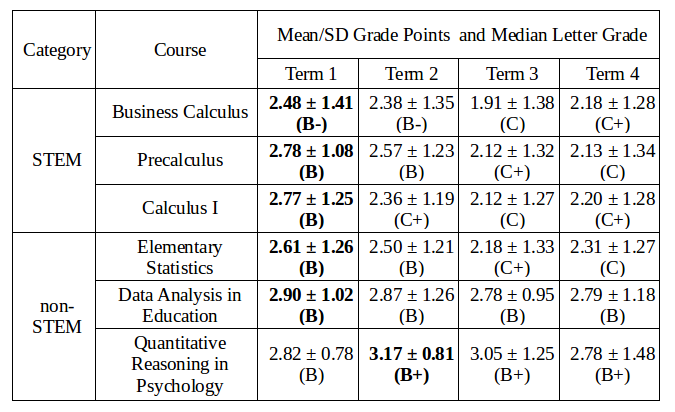
\includegraphics[width=0.49\textwidth]{tables/table_math_grades.png}
\label{table_math_grades}
\end{table}

To more clearly depict the mean, median, and spread of the Math course grades in the context of when each course was taken, Figures \ref{Math_STEM_courses} and \ref{Math_nonSTEM_courses} show boxplots of the grades, with the mean value annotated with text and a horizontal line through each bar.  

\begin{figure}[htbp]
\centering
    \begin{subfigure}[b]{0.31\textwidth}
    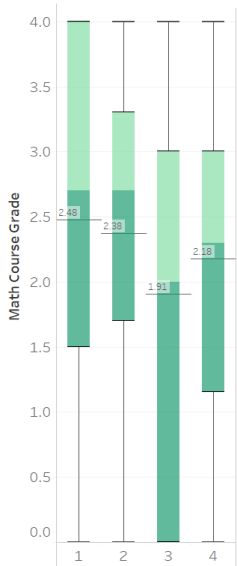
\includegraphics[width=\textwidth]{root/figures/revmath110.png}
    \centering
    \caption{Business Calculus}
    \end{subfigure}
    \hspace{2mm}
    \begin{subfigure}[b]{0.31\textwidth}
    \centering
    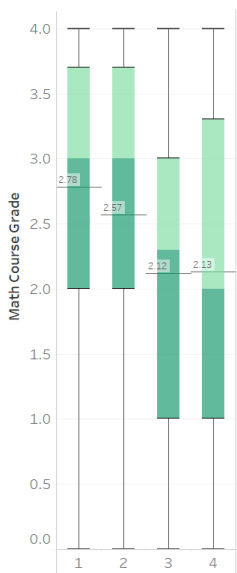
\includegraphics[width=\textwidth]{root/figures/revmath199.png}
    \caption{Precalculus}
    \end{subfigure}
    \hspace{2mm}
    \begin{subfigure}[b]{0.31\textwidth}
    \centering
    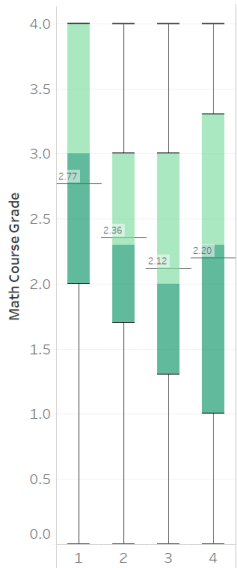
\includegraphics[width=\textwidth]{root/figures/revmath226.png}
    \caption{Calculus I}
    \end{subfigure}
\caption{Math course performance in STEM courses.}
\label{Math_STEM_courses}
\end{figure}

\begin{figure}[htbp]
\centering
    \begin{subfigure}[b]{0.3\textwidth}
    \centering
    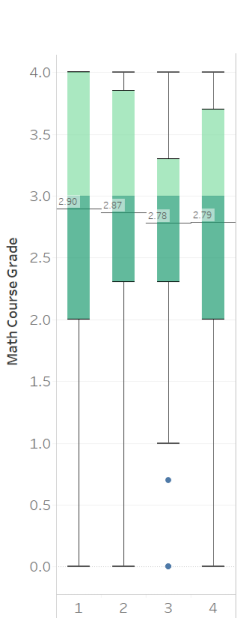
\includegraphics[width=\textwidth]{root/figures/revised160.png}
    \caption{Data Analysis in Education}
    \end{subfigure}
    \hspace{4mm}
    \begin{subfigure}[b]{0.3\textwidth}
    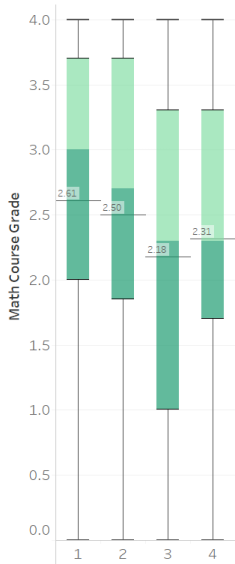
\includegraphics[width=\textwidth]{root/figures/revmath124.png}
    \centering
    \caption{Introductory Statistics \\  \hspace{2mm} }
    \end{subfigure}
    \hspace{4mm}
    \begin{subfigure}[b]{0.3\textwidth}
    \centering
    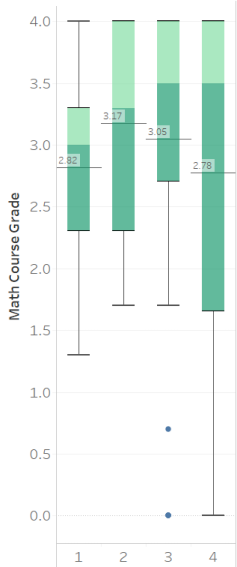
\includegraphics[width=\textwidth]{root/figures/revpsy171.png}
    \caption{Quantitative Reasoning \\  \hspace{2mm}}
    \end{subfigure}
\caption{Math course performance in non-STEM courses.}
\label{Math_nonSTEM_courses}
\end{figure}

For each Math course, students who took the Math course in the first year (terms 1 or 2) had the highest mean grade.  The effect was most pronounced in the Calculus I course, where the mean grade of 2.77 for students who took it in term 1 was 0.65 or 0.57 grade points higher than the students in term 3 or term 4 respectively. Overall, the extent of the advantage for students to take the Math course in the first year was greater for STEM courses than for the non-STEM courses.  However, for all six courses, the highest mean grade points achieved in the course was within one standard deviation of the lowest mean grade, indicating that the term in which the Math course was taken did not have a pronounced effect on the grade in the course.  

We then examined whether taking the Math course in the first versus second year of a student's curriculum led to higher fifth-term persistence, seventh-term persistence, or graduation rates (Table \ref{table:math_outcomes}).  The research revealed statistically significant evidence ($\alpha$ = 0.05) that the fifth-term persistence and seventh-term persistence of students who took their STEM or non-STEM Math course in the second year (i.e., third or fourth semester) were higher than that of students who took the Math course in their first year.  However, there was no statistically significant evidence that the graduation rate of the students who took their Math course in the first year was different than that of the students who took their Math course in the second year.  Overall, these rates can potentially inform the advising and curriculum-planning strategies utilized for entering students, to the effect that delaying the onset of the Math courses until the second year can lead to higher fifth-term and seventh-term persistence.  

However, these results also highlight the difficulty in attempting to predict a student's long-term outcome based on the performance in a single course taken in the first two years, since Table \ref{table_math_grades} indicates that students get higher Math grades in the first year.  These results suggest that performance in a single course is too narrow a view of the student's academic curriculum for predicting persistence or graduation.

Accordingly, the next section expands the scope of the analysis of student academic data to the curriculum level, examining the extent of progress through the foundation course sequences rather than focusing on a single course. 

\begin{table}[htbp]
\centering
\caption{Persistence and graduation of students in relation to the timing of Math courses.}
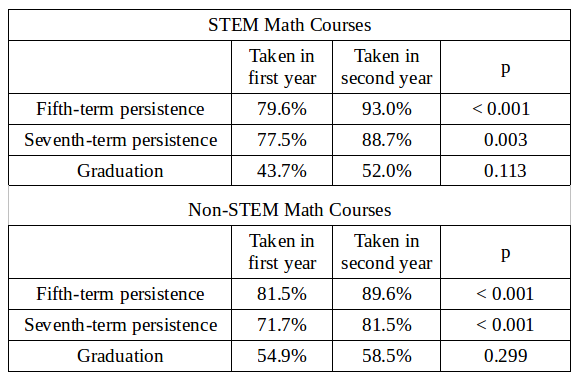
\includegraphics[width=0.5\textwidth]{tables/math_outcomes.png}
\label{table:math_outcomes}
\end{table}


\section{Progress through Foundation Course Sequences}
\label{results_prescribedpatterns}

The results presented in this section assess the foundation course sequences of the Metro program, rather than focusing on individual courses as in the preceding subsection. Recall that each student in the two-year program is required to take a 3-course foundation sequence (Figure \ref{capstone}).  We determined each student's progress through this sequence and aggregated the results by this ``core-progress" value across all students.

\begin{figure}[htbp]
    \centering
    \begin{subfigure}[b]{\textwidth}
    \centering
    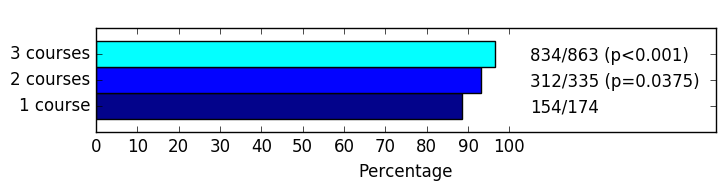
\includegraphics[width=0.9\textwidth]{figures/pathways_fifthpers.png}
    \caption{Fifth-Term Persistence}
    \label{pathways_fifth}
    \vspace{6mm}
    \end{subfigure}
    \begin{subfigure}[b]{\textwidth}
    \centering
    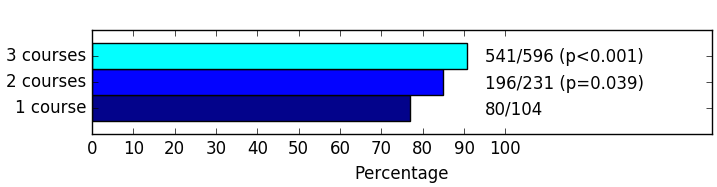
\includegraphics[width=0.9\textwidth]{figures/pathways_seventhpers.png}
    \caption{Seventh-Term Persistence}
    \label{pathways_seventh}
    \vspace{6mm}
    \end{subfigure}
    \vspace{6mm}
    \begin{subfigure}[b]{\textwidth}
    \centering
    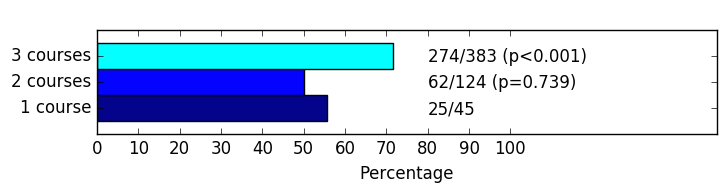
\includegraphics[width=0.9\textwidth]{figures/pathways_grad.png}
    \caption{Graduation}
    \label{pathways_grad}
    \end{subfigure}
\caption{Fifth and seventh-term persistence and graduation rates by extent of foundation course sequence completion.  Each bar is annotated with the raw data that yielded the percentage, and with the p-value for the hypothesis that the percentage represented by that bar is greater than the one below it.}
\label{core_pathway_outcomes}
\end{figure}

The results for the foundation course sequence analysis are shown in Figure \ref{core_pathway_outcomes}.  The analysis revealed statistically significant evidence that fifth-term and seventh-term persistence percentages are higher for students who completed all three of the foundation courses, compared to the students who complete only two.  Likewise, students who complete two of the courses have higher fifth-term and seventh-term persistence than students who complete only one course in the foundation course sequence.  For graduation, students who complete the entire foundation course sequence had the highest graduation rate, while students who completed only one course had a higher graduation rate than students who completed two.  The latter is an interesting finding, though it is worth noting that the sample size of the 1-course group for the graduation analysis (45 students total) is relatively small, because the vast majority of the students who participate in the Metro program complete their foundation course sequence.  

The next step in the analysis was to determine whether the pattern revealed by Figure \ref{core_pathway_outcomes}, in which students who complete all three foundation courses had greater persistence and graduation rates than student who complete fewer of the courses, could be observed even when students are categorized based on different demographic and socioeconomic characteristics.  Thus, students with different core progress values were further divided into different groups based on gender, race, and Pell eligibility, and the fifth-term persistence, seventh-term persistence, and graduation percentages of each group was compared, as shown in the figures that follow.

Figures \ref{fifth_progress_gender}-\ref{grad_progress_gender} reveal that male and female students both presented the same pattern as the prior findings of Figure \ref{core_pathway_outcomes}: students who make the full three-course progress through the foundation course sequences had higher persistence and graduation percentages than students who made less progress, within each gender.  With respect to fifth-term and seventh-term persistence, students who took only two of the courses had higher persistence rates than students who took only one, again within each gender.  

\begin{figure}[htbp]
\centering
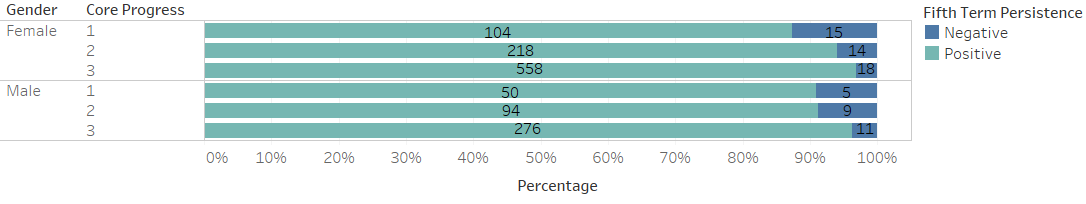
\includegraphics[width=0.98\textwidth]{root/figures/FifthProgressGender.png}
\caption{Fifth-term persistence by core progress value of Metro students, across genders.  Each bar is annotated with the counts of student with positive and negative values of the persistence or graduation outcome.}
\label{fifth_progress_gender}
\end{figure}

\begin{figure}[htbp]
\centering
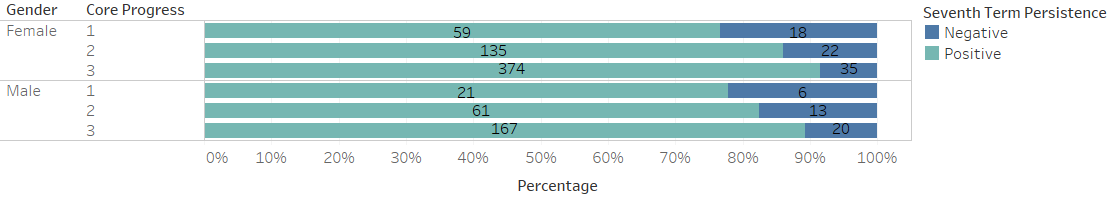
\includegraphics[width=0.98\textwidth]{root/figures/SeventhProgressGender.png}
\caption{Seventh-term persistence by core progress value of Metro students, across genders.  Each bar is annotated as in Figure \ref{fifth_progress_gender}.}
\label{seventh_progress_gender}
\end{figure}

\begin{figure}[htbp]
\centering
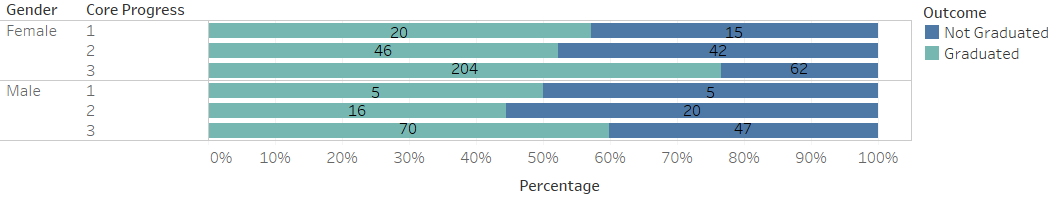
\includegraphics[width=0.98\textwidth]{root/figures/GradProgressGender.png}
\caption{Graduation outcome by core progress value of Metro students, across genders.  Each bar is annotated as in Figure \ref{fifth_progress_gender}.}
\label{grad_progress_gender}
\end{figure}

Likewise, Figures \ref{fifth_progress_race}-\ref{grad_progress_race} indicate that within each race category, students who complete all three of the foundation courses generally have higher persistence and graduation rates than students who complete fewer of the courses.  Deviations from this pattern occur in those instances where the group sizes are very small, because only a very small number of students complete only a single course.   

\begin{figure}[htbp]
\centering
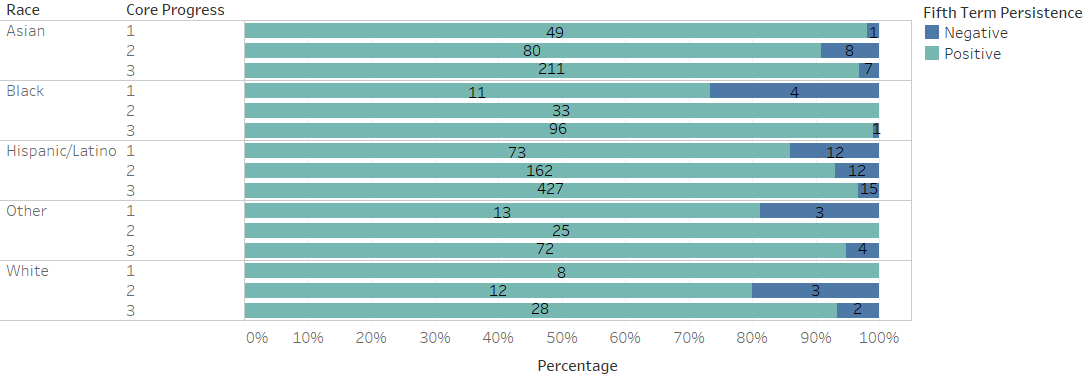
\includegraphics[width=0.98\textwidth]{root/figures/FifthProgressRace.png}
\caption{Fifth-term persistence by core progress value of Metro students, across races. Each bar is annotated as in Figure \ref{fifth_progress_gender}.}
\label{fifth_progress_race}
\end{figure}

\begin{figure}[htbp]
\centering
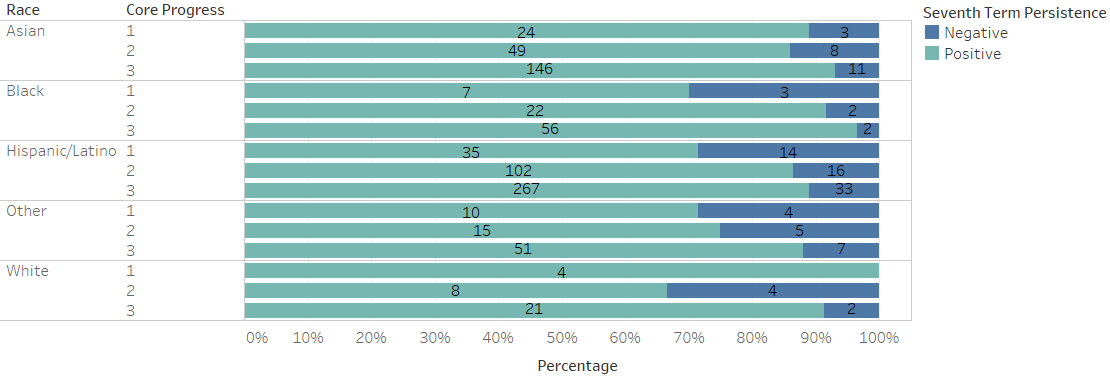
\includegraphics[width=0.98\textwidth]{root/figures/SeventhProgressRace.png}
\caption{Seventh-term persistence by core progress value of Metro students, across races.  Each bar is annotated as in Figure \ref{fifth_progress_gender}.}
\label{seventh_progress_race}
\end{figure}

\begin{figure}[htbp]
\centering
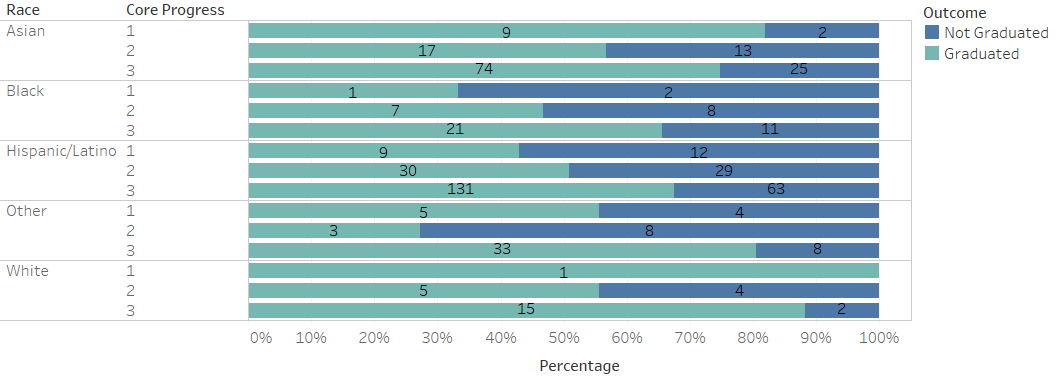
\includegraphics[width=0.98\textwidth]{root/figures/GradProgressRace.png}
\caption{Graduation outcome by core progress value of Metro students, across races.  Each bar is annotated as in Figure \ref{fifth_progress_gender}.}
\label{grad_progress_race}
\end{figure}

Lastly, Figures \ref{fifth_progress_pell}-\ref{grad_progress_pell} demonstrate that the effect of greater extent through the foundation course sequences is also observed within students with or without Pell eligibility.  Thus, once again, the effect of increased progress through the foundation course sequences is observed in students regardless of their Pell eligibility.  

\begin{figure}[htbp]
\centering
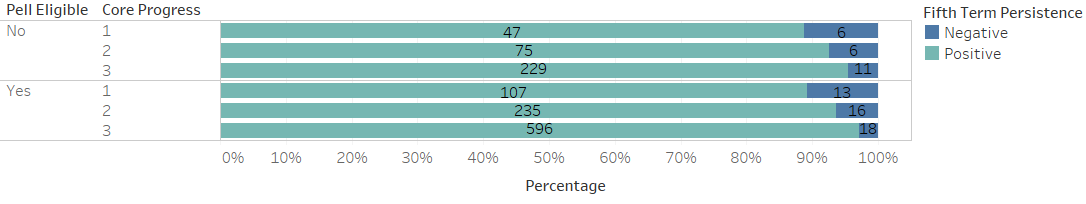
\includegraphics[width=0.98\textwidth]{root/figures/FifthProgressPell.png}
\caption{Fifth-term persistence by core progress value of Metro students, by Pell eligibility. Each bar is annotated as in Figure \ref{fifth_progress_gender}.}
\label{fifth_progress_pell}
\end{figure}

\begin{figure}[htbp]
\centering
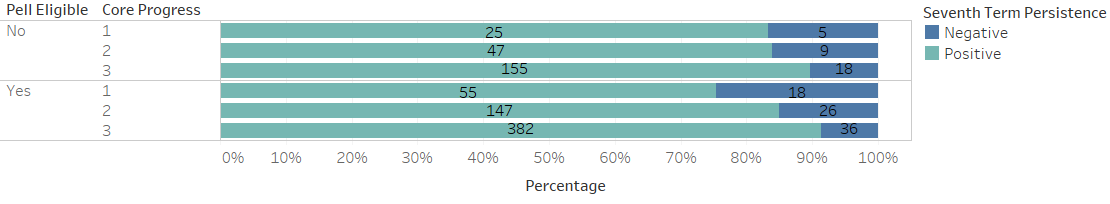
\includegraphics[width=0.98\textwidth]{root/figures/SeventhProgressPell.png}
\caption{Seventh-term persistence by core progress value of Metro students, by Pell eligibility.  Each bar is annotated as in Figure \ref{fifth_progress_gender}.}
\label{seventh_progress_pell}
\end{figure}

\begin{figure}[htbp]
\centering
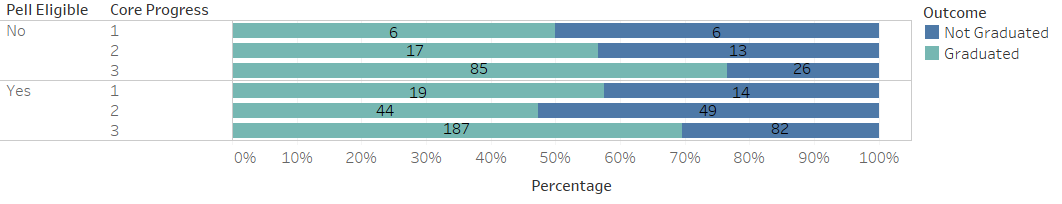
\includegraphics[width=0.98\textwidth]{root/figures/GradProgressPell.png}
\caption{Graduation outcome by core progress value of Metro students, by Pell eligibility.  Each bar is annotated as in Figure \ref{fifth_progress_gender}.}
\label{grad_progress_pell}
\end{figure}

The foregoing results demonstrate that the extent of a student's progress through their chosen course sequences offers potential for predicting a student's graduation likelihood, even within categories of students based on different demographic, personal, and socioeconomic features such as gender, race, and Pell eligibility.  

In the next section, the examination of this section is extended to encompass the course sequences most frequently taken by students in the pool consisting of the Metro program and the control group collectively.   In so doing, we assess whether increased progress through the course sequences extracted via sequential pattern mining exhibits a similar effect on persistence and graduation rates.  


\section{Sequential Patterns and Progress through Sequences}
\label{results_chosensequences}

The results presented in this section assess whether progress through course sequences extracted via sequential pattern mining exhibits the same effect on persistence and graduation as did progress through the Metro program's foundation course sequences, as described in the previous section.  

The number of distinct sequences that were mined from the student records from (1) the participants in the Metro program, and (2) the participants of the program combined with the associated control group, are shown in Tables \ref{minsup_length_metro} and \ref{minsup_length_metrocomp} respectively. Next, the number of distinct sequences mined from all the student records in the dataset is shown in Table \ref{minsup_length_all}.  The Tables reveal that the number of distinct sequences increases as the required minimum support was decreased.  Likewise, increasing the minimum sequential pattern length leads to a decrease in the number of number of distinct sequences identified, except for the transition of minimum sequence length of 2 to 3 courses at a minimum support of 0.01.  This trend may have arisen due to the increased number of possible combinations of courses of length 3 compared to length 2, along with the minimum support being reduced to its lowest value of 0.01. 

Tables \ref{minsup_length_metro}-\ref{minsup_length_all} collectively reveal that the number of students in the underlying course sequence data has a significant effect on the number of sequential patterns extracted at each minimum sequence length and support threshold. As the number of students increases to the full dataset in \ref{minsup_length_all}, the number of mined sequential patterns increases, but the proportion of students to whom any particular mined pattern relates decreases, with the result that the mined sequences, while more numerous, are less informative.  As discussed in more detail in Chapter \ref{Chapter_Discussion}, these findings suggest that sequential pattern mining is best suited to situations where a large fraction of the students are expected to have similar sequences (e.g., students within a department or major).  In the following sections, the analysis proceeds with the student pool consisting of the Metro program participants and the control group, as shown in Table \ref{minsup_length_metrocomp}, because it offers the best compromise between a large number of extracted sequences and a relatively small number of students to whom the sequences pertain.   

\begin{table}[htbp]
\centering
\caption{Number of distinct sequences, Metro program participants.}
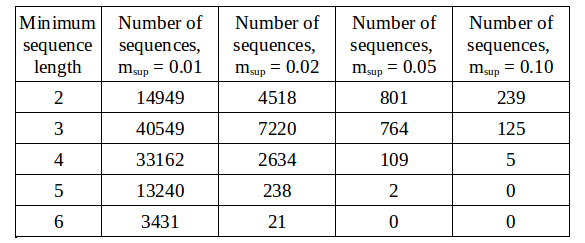
\includegraphics[width=0.75\textwidth]{tables/minsup_length_metro.png}
\label{minsup_length_metro}
\end{table}

\begin{table}[htbp]
\centering
\caption{Number of distinct sequences, Metro participants and control group.}
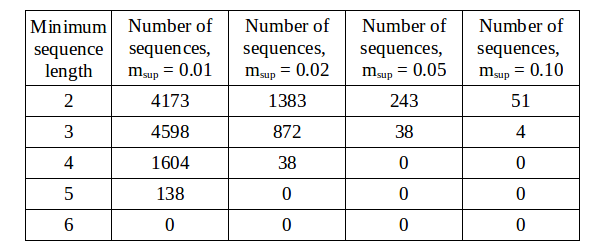
\includegraphics[width=0.75\textwidth]{tables/minsup_length_metrocomp.png}
\label{minsup_length_metrocomp}
\end{table}

\begin{table}[htbp]
\centering
\caption{Number of distinct sequences, entire dataset of Table \ref{table:students}.}
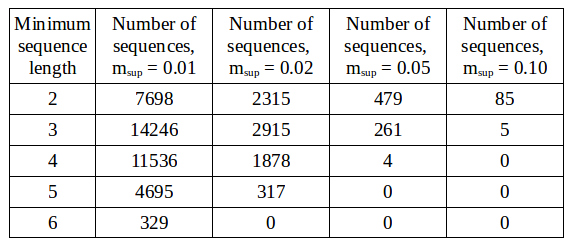
\includegraphics[width=0.75\textwidth]{tables/minsup_all.png}
\label{minsup_length_all}
\end{table}

The top ten most frequently-taken course sequences of length 3 were aggregated across sequences by progress value, as described more fully in the Methods section.  Figure \ref{agg_top3} shows the fifth-term persistence, seventh-term persistence, and graduation percentages for each progress value, aggregated across the top ten length-3 sequential patterns for the Metro program and control group students collectively.  Likewise, Figure \ref{agg_top5} shows the seventh-term persistence, and graduation percentages for each progress value, aggregated across the top five length-5 sequential patterns for the program and control group students.  Each of the bars is annotated with the raw data that yielded the shown percentages.  Furthermore, each bar is annotated with a p value for the hypothesis that the percentage reflected by a certain bar is greater than the bar below it.  

\begin{figure}[htbp]
\centering
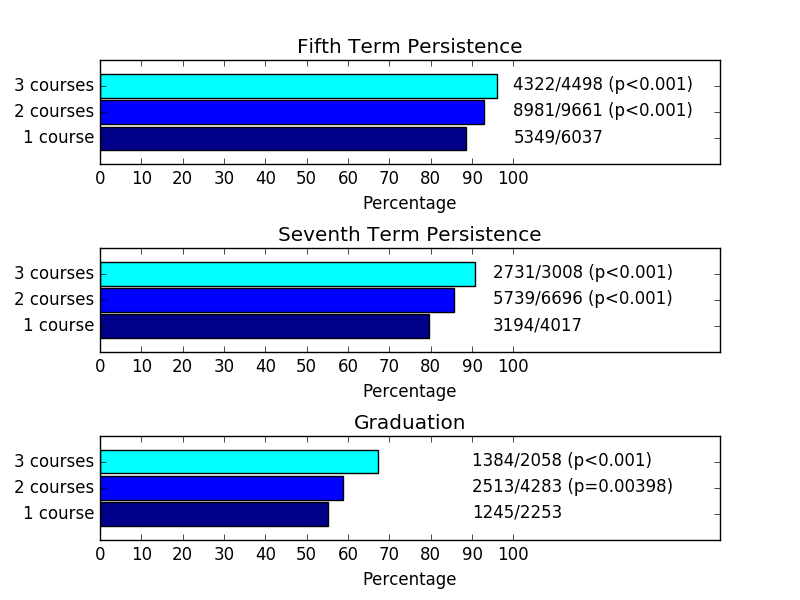
\includegraphics[width=0.9\textwidth]{figures/agg_top3_metrocomp.png}
\caption{Persistence and graduation rates by extent of completion of the ten most-frequently taken length-3 course sequences.  Each bar is annotated with the raw data that yielded the percentage, and with the p-value for the hypothesis that the percentage represented by that bar is greater than the one below it.}
\label{agg_top3}
\end{figure}

Figure \ref{agg_top3} reveals that students who make increasing progress through their chosen sequence have higher persistence and graduation rates than those who make less progress through those same sequences.  The same bar graphs for each of the ten individual length-3 sequences revealed the same trend.  The p values shown at the far right of each bar indicate that the analysis has yielded statistically significant evidence that the fifth-term persistence, seventh-term persistence, and graduation rates of students who completed 3 courses are higher than those of students who completed only 2 courses (and likewise for the students who completed 2 courses versus 1 course). 

The analysis for the length-5 sequential patterns, shown in Figure \ref{agg_top5}, reveal a similar trend as the length-3 patterns. For seventh-term persistence, students who make increased progress through the sequences (e.g., 5 courses versus 4, and so on) have higher persistence percentages than those who make less progress.  For graduation, the analysis revealed that students who make the full 5-course progress through their sequences enjoyed higher graduation rates than students who took four, and likewise for four versus three. However, there was no statistically significant evidence that students who complete three courses have higher graduation rates than students who take two, and so on.

\begin{figure}[htbp]
\centering
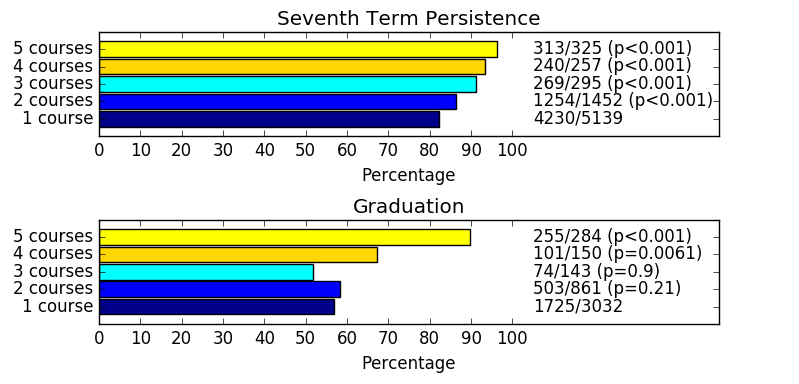
\includegraphics[width=\textwidth]{figures/agg_top5_metrocomp.png}
\caption{Seventh-term persistence and graduation rates by extent of completion of the five most frequently taken length-5 course sequences.  Each bar is annotated in the same way as in Figure \ref{agg_top3}.}
\label{agg_top5}
\end{figure}

In Figures \ref{agg_top3} and \ref{agg_top5}, the top ten and top five most common sequences, respectively, were aggregated to produce a high-level picture of the effect that progress through sequences had on persistence and graduation.  The next two subsections consider the this subsection, we examined the most frequently-encountered course sequences mined in an unsupervised fashion from the student data.  In the next subsection, the most common length-3 and length-5 sequences are examined in more detail.   

\subsection{Progress through the Most Common Length-3 Sequences}

The top ten most frequently taken three-course sequences are shown in Figure \ref{length3top10}.  

\begin{figure}[htbp]
\centering
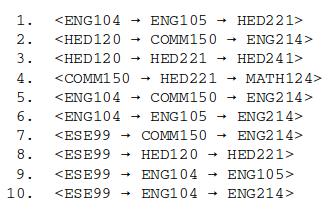
\includegraphics[width=0.5\textwidth]{root/figures/length3top10.png}
\caption{Most frequently taken length-three course sequences.}
\label{length3top10}
\end{figure}

The series of graphs that follows shows the percentage of students who persisted and graduated as a function of the number of courses from the sequences of Figure \ref{length3top10} that were completed by each student.

\begin{figure}[!htbp]
\centering
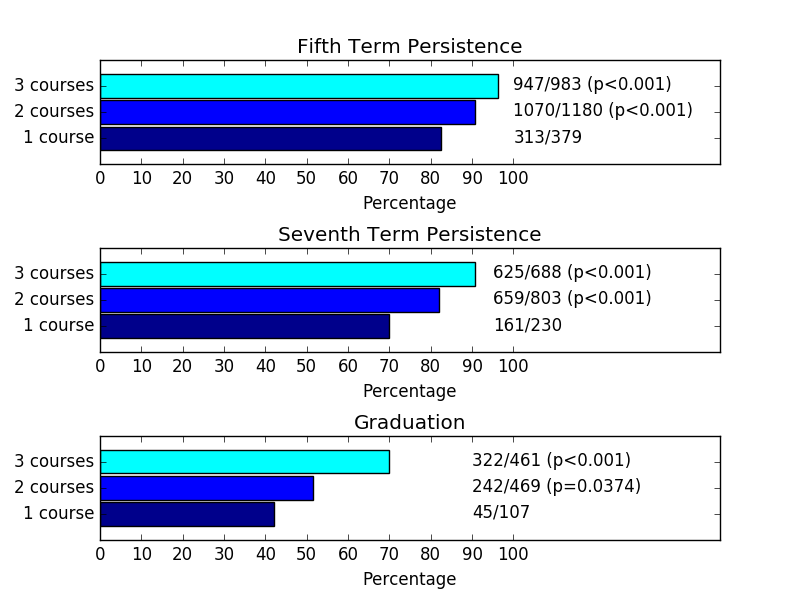
\includegraphics[height=7cm]{root/figures/length3/seq3_1_progress.png}
\caption{Fifth-term and seventh-term persistence and graduation by extent of number of courses completed in length-3 Sequence 1.}
\label{seq3_1}
\end{figure}

\begin{figure}[!htbp]
\centering
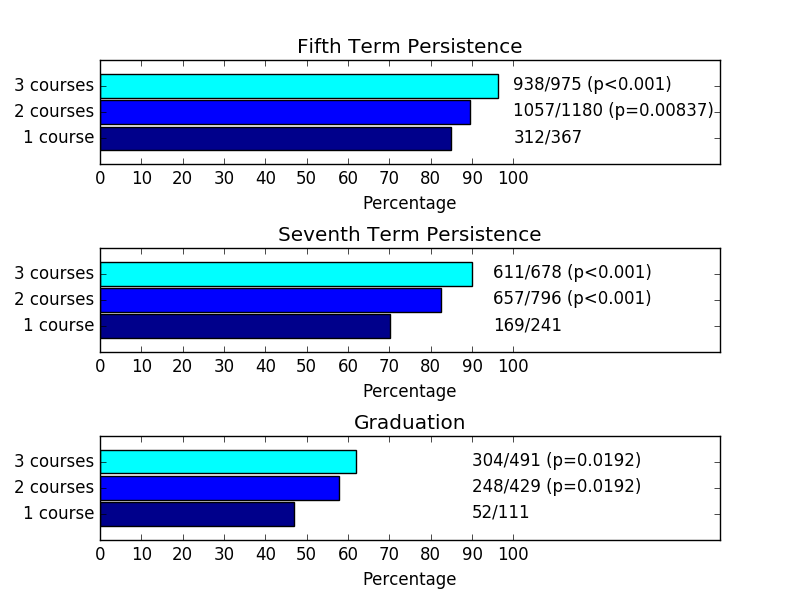
\includegraphics[height=7cm]{root/figures/length3/seq3_2_progress.png}
\caption{Fifth-term and seventh-term persistence and graduation by extent of number of courses completed in length-3 Sequence 2.}
\label{seq3_2}
\end{figure}

\begin{figure}[!htbp]
\centering
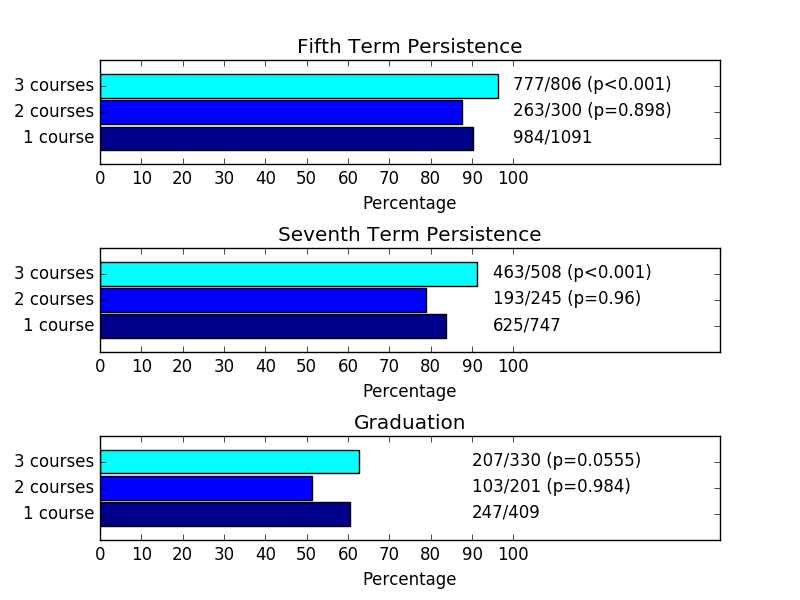
\includegraphics[height=7cm]{root/figures/length3/seq3_3_progress.png}
\caption{Fifth-term and seventh-term persistence and graduation by extent of number of courses completed in length-3 Sequence 3.}
\label{seq3_3}
\end{figure}

\begin{figure}[!htbp]
\centering
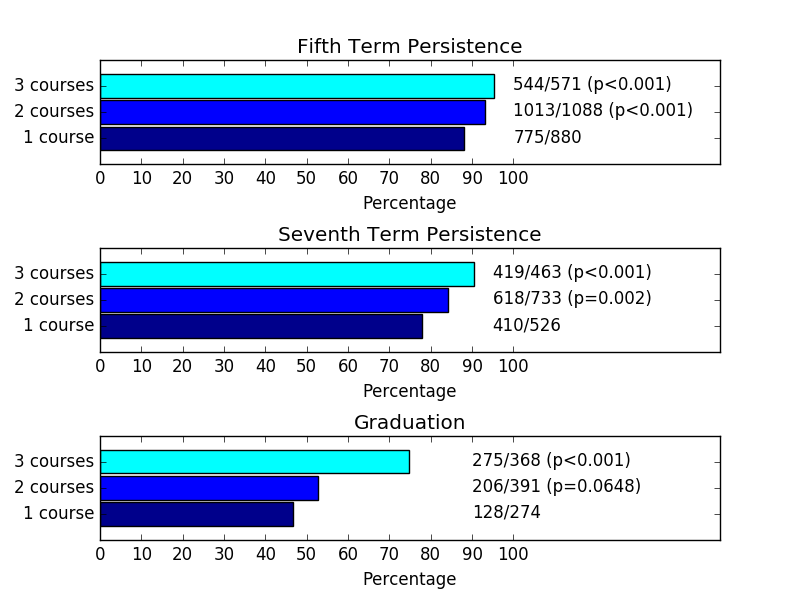
\includegraphics[height=7cm]{root/figures/length3/seq3_4_progress.png}
\caption{Fifth-term and seventh-term persistence and graduation by extent of number of courses completed in length-3 Sequence 4.}
\label{seq3_4}
\end{figure}

\begin{figure}[!htbp]
\centering
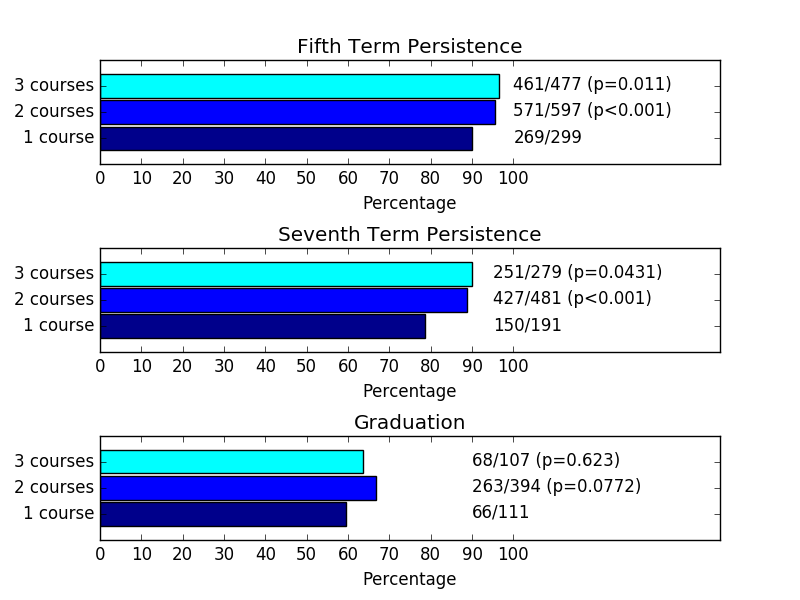
\includegraphics[height=7cm]{root/figures/length3/seq3_5_progress.png}
\caption{Fifth-term and seventh-term persistence and graduation by extent of number of courses completed in length-3 Sequence 5.}
\label{seq3_5}
\end{figure}

\begin{figure}[!htbp]
\centering
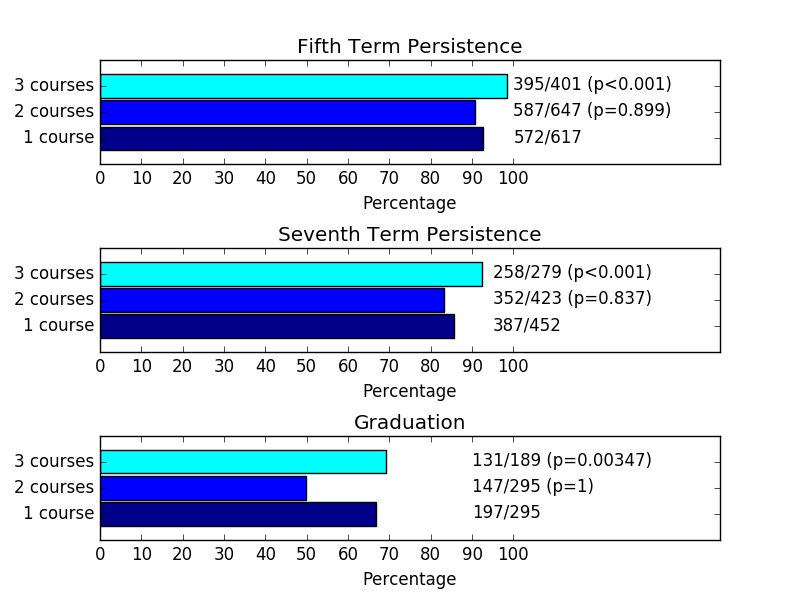
\includegraphics[height=7cm]{root/figures/length3/seq3_6_progress.png}
\caption{Fifth-term and seventh-term persistence and graduation by extent of number of courses completed in length-3 Sequence 6.}
\label{seq3_6}
\end{figure}

\begin{figure}[!htbp]
\centering
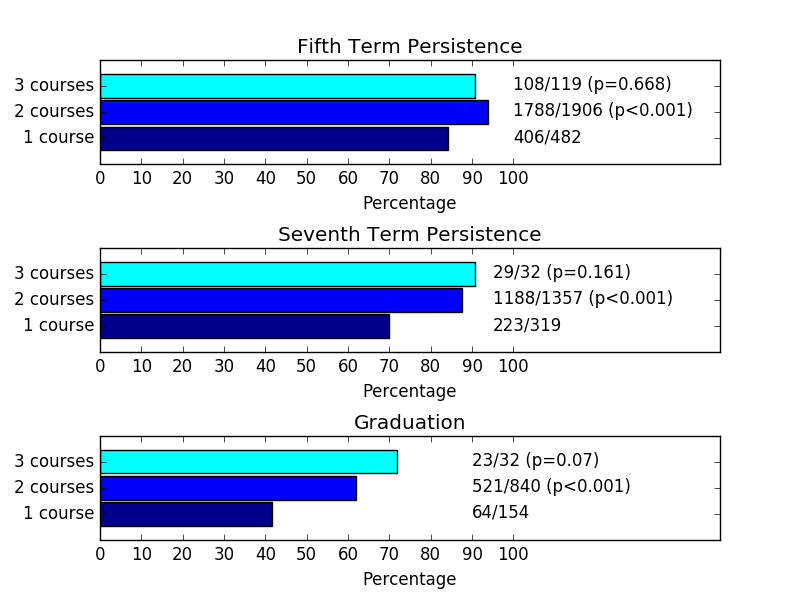
\includegraphics[height=7cm]{root/figures/length3/seq3_7_progress.png}
\caption{Fifth-term and seventh-term persistence and graduation by extent of number of courses completed in length-3 Sequence 7.}
\label{seq3_7}
\end{figure}

\begin{figure}[!htbp]
\centering
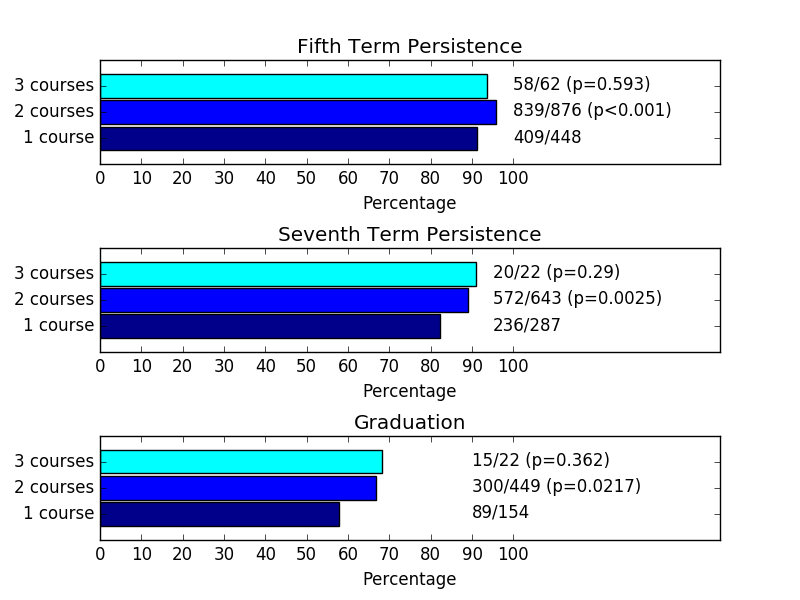
\includegraphics[height=7cm]{root/figures/length3/seq3_8_progress.png}
\caption{Fifth-term and seventh-term persistence and graduation by extent of number of courses completed in length-3 Sequence 8.}
\label{seq3_8}
\end{figure}

\begin{figure}[!htbp]
\centering
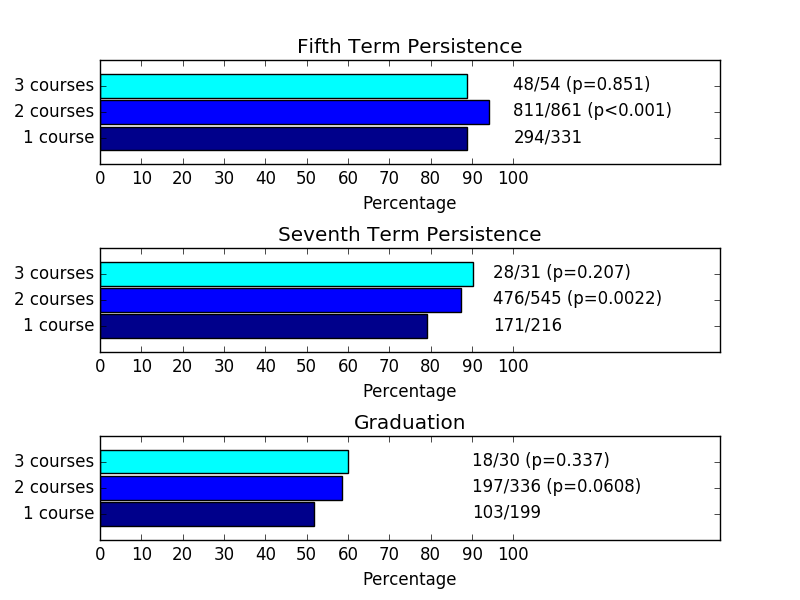
\includegraphics[width=0.7\textwidth]{root/figures/length3/seq3_9_progress.png}
\caption{Fifth-term and seventh-term persistence and graduation by extent of number of courses completed in length-3 Sequence 9.}
\label{seq3_9}
\end{figure}

\begin{figure}[!htbp]
\centering
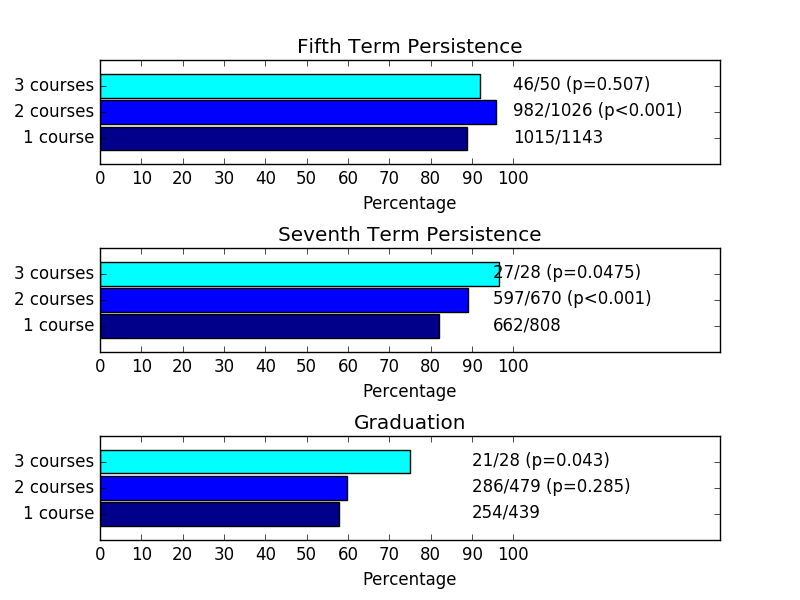
\includegraphics[width=0.7\textwidth]{root/figures/length3/seq3_10_progress.png}
\caption{Fifth-term and seventh-term persistence and graduation by extent of number of courses completed in length-3 Sequence 10.}
\label{seq3_10}
\end{figure}



\pagebreak
\subsection{Progress through the Most Common Length-5 Sequences}

The top ten most frequently taken five-course sequences are shown in Figure \ref{length5top5}.  

\begin{figure}[htbp]
\centering
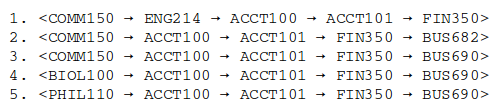
\includegraphics[width=0.8\textwidth]{root/figures/length5top5.png}
\caption{Most frequently taken length-five course sequences.}
\label{length5top5}
\end{figure}

The series of graphs that follows shows the percentage of students who persisted and graduated as a function of the number of courses from the sequences of Figure \ref{length5top5} that were completed by each student.

\begin{figure}[htbp]
\centering
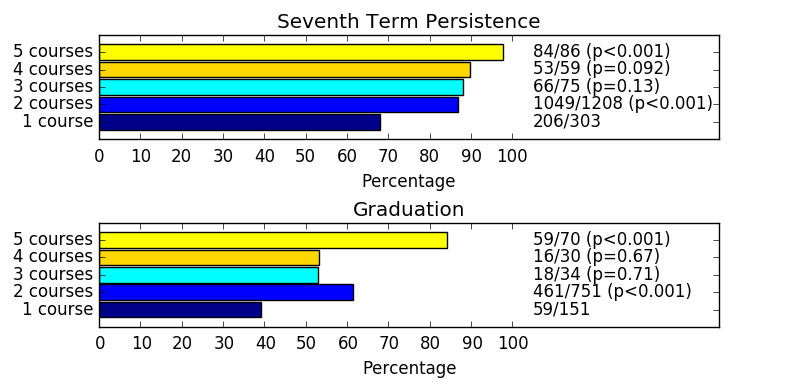
\includegraphics[width=0.8\textwidth]{root/figures/length5/seq5_1_progress.png}
\caption{Seventh-term persistence and graduation by extent of number of courses completed in length-5 Sequence 1.}
\label{seq5_1}
\end{figure}

\begin{figure}[htbp]
\centering
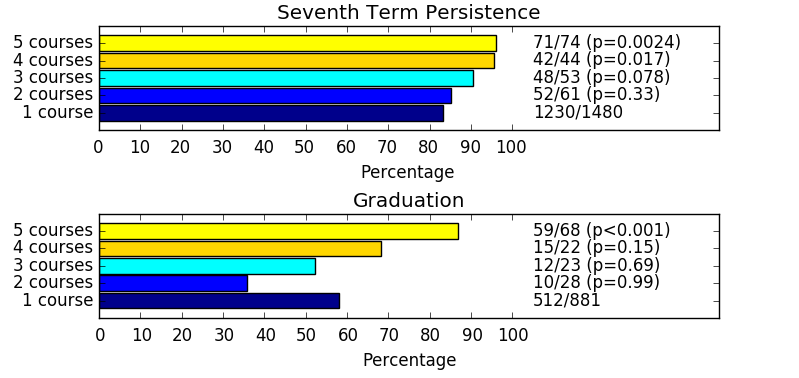
\includegraphics[width=0.8\textwidth]{root/figures/length5/seq5_2_progress.png}
\caption{Seventh-term persistence and graduation by extent of number of courses completed in length-5 Sequence 2.}
\label{seq5_2}
\end{figure}

\begin{figure}[htbp]
\centering
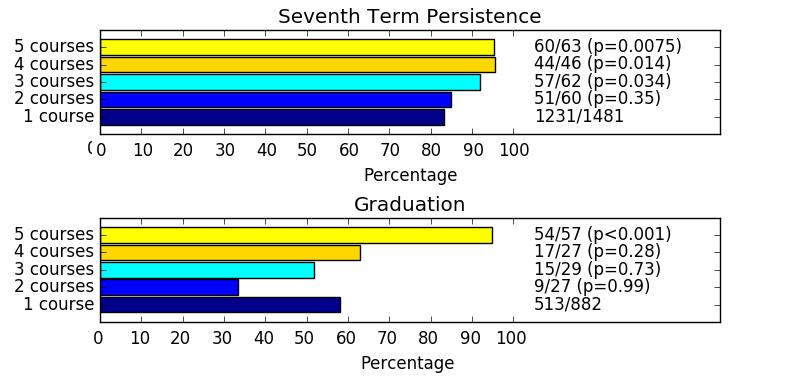
\includegraphics[width=0.8\textwidth]{root/figures/length5/seq5_3_progress.png}
\caption{Seventh-term persistence and graduation by extent of number of courses completed in length-5 Sequence 3.}
\label{seq5_3}
\end{figure}

\begin{figure}[htbp]
\centering
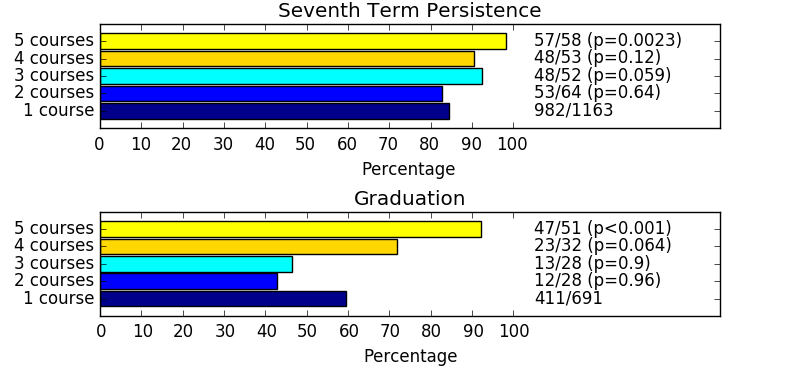
\includegraphics[width=0.8\textwidth]{root/figures/length5/seq5_4_progress.png}
\caption{Seventh-term persistence and graduation by extent of number of courses completed in length-5 Sequence 4.}
\label{seq5_4}
\end{figure}

\begin{figure}[htbp]
\centering
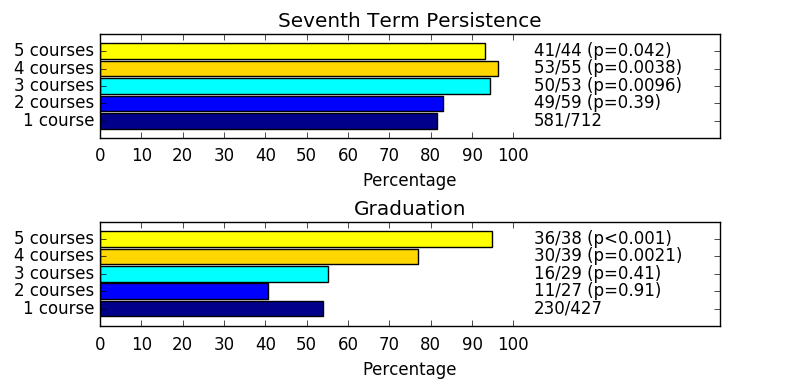
\includegraphics[width=0.8\textwidth]{root/figures/length5/seq5_5_progress.png}
\caption{Seventh-term persistence and graduation by extent of number of courses completed in length-5 Sequence 5.}
\label{seq5_5}
\end{figure}

The prior sections have demonstrated that the progress made by students through their prescribed (in the case of the foundation course sequences) or chosen (in the case of the most frequent sequences of three or five courses) sequences are predictive of students' likelihood to persist and graduate.  Figures \ref{agg_top3} and \ref{agg_top5} reveal the same pattern as Figures \ref{fifth_progress_gender}-\ref{grad_progress_pell}, in that students who take all the courses in their chosen length-3 or length-5 sequences have higher persistence and graduation rates than students who take fewer of those courses.  As such, the analysis of Section \ref{results_prescribedpatterns}, in which students were further categorized by certain demographic features such as race, gender and Pell eligibility, was not repeated with the sequences extracted via sequential pattern mining in this section.

The next section reveals and interprets the findings as to whether fifth-term and seventh-term persistence are stronger features for predicting graduation than other demographic, socioeconomic, and personal factors, such as a student's race, gender, Pell eligibility, and ELM and EPT entrance scores. 

\section{Feature Importance and Recursive Feature Elimination}
\label{results_section_featureimportance}

The first step in the feature importance comparison was to assess the accuracy of naive Bayes, logistic regression, and random forest classification models for predicting graduation status of students using all available features (Table \ref{feature_sets}, left column) for the student pool consisting of the Metro program participants and their control group counterparts.  Boxplots for the resulting accuracy scores are shown in Figure \ref{accuracies_all}.  The mean and standard deviation of the accuracy scores (Table \ref{table_accuracies}) reveal that the accuracy scores are within one standard deviation of each other, with no one model showing significantly better performance than the others.  The random forest model's Gini importance values for the top six most important features (Figure \ref{featureimportances_all}) indicate that the seventh-term persistence was the most influential feature.  The parents' education levels had the next highest importance values.  Race and gender were not among the top six features.   

\begin{figure}[htbp]
\centering
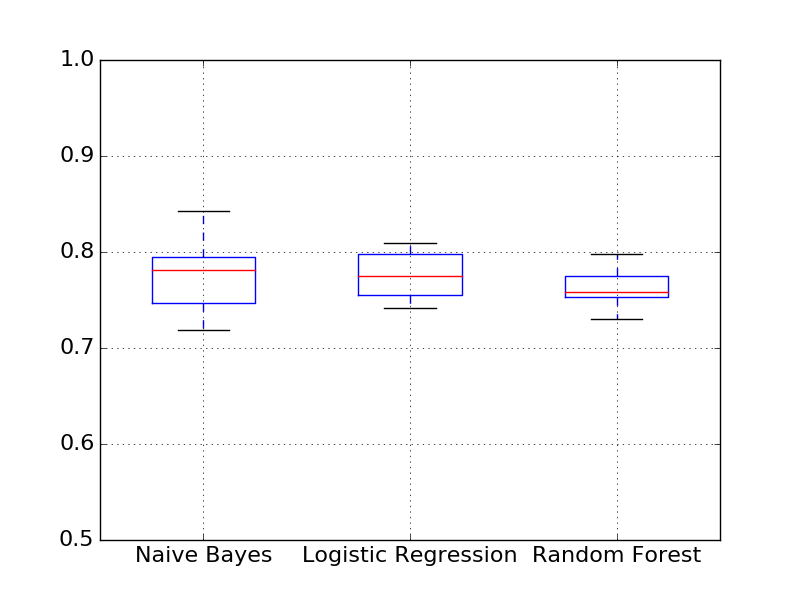
\includegraphics[width=0.75\textwidth]{figures/accuracies_all_metrocomp.png}
\caption{Accuracy of naive Bayes, logistic regression, and random forest classification models.}
\label{accuracies_all}
\end{figure}

\begin{figure}[htbp]
\centering
\includegraphics[width=\textwidth]{figures/featureimportances_all.png}
\caption{Top six Gini importance measures for the random forest classifier, using all available features.}
\label{featureimportances_all}
\end{figure}

\begin{table}[htbp]
\centering
\caption{All features (left column) and features resulting from RFE (right column).}
\includegraphics[width=0.5\textwidth]{tables/feature_sets.png}
\label{feature_sets}
\end{table}

\begin{table}[htbp]
\centering
\caption{Mean and standard deviation of accuracy scores with (a) the original feature set, and (b) the feature set after recursive feature elimination (RFE).}
\includegraphics[width=0.75\textwidth]{tables/table_accuracies.png}
\label{table_accuracies}
\end{table}

Recursive feature elimination (RFE) reduced the features used in the classification models to those listed in Table \ref{feature_sets}, right column.  The accuracy scores of each model type with the reduced feature set is shown in Figure \ref{accuracies_reduced}.  As shown there and in the right-hand column of Table \ref{table_accuracies}, the accuracy of the random forest model improved the most significantly after reduction of the feature set to exclude the least useful features.  Meanwhile,  seventh-term persistence had the highest Gini importance of the features that remained after recursive feature elimination (Figure \ref{importances_reduced}).  For both the full and the RFE-reduced feature sets, it can be observed that seventh-term persistence outweighs other personal factors such as race, gender, or entrance scores, in being able to predict graduation.    

\begin{figure}[htbp]
\centering
\includegraphics[width=0.75\textwidth]{figures/accuracies_reduced.png}
\caption{Accuracy of naive Bayes, logistic regression, and random forest classification models, after recursive feature elimination.}
\label{accuracies_reduced}
\end{figure}

\begin{figure}[htbp]
\centering
\includegraphics[width=\textwidth]{figures/importances_reduced.png}
\caption{Gini importance measures for the random forest classifier, after recursive feature elimination.}
\label{importances_reduced}
\end{figure}

The importance of seventh-term persistence as a feature in the random forest model for predicting graduation may seem unsurprising: after all, a student with positive seventh-term persistence has made almost complete progress towards graduation, so it follows logically that seventh-term persistence would be revealed as an important feature for predicting graduation.  However, the fact that the best accuracy of the random forest classifier after recursive feature elimination is 78.7\% highlights the complexity of the problem of predicting whether a student will graduate: even students with positive seventh-term persistence have a substantial likelihood of not graduating.  

As Table \ref{seventh_and_grad} shows, of the students from the 2009-2013 cohorts with positive seventh-term persistence, only 76.5\% of those students graduated overall.  Interestingly, the percentage was higher for Metro students than for comparison students, but the difference was not statistically significant (78.3\% vs 74.0\%, p = 0.13).  Thus, Metro students who have persisted for seven terms are more likely to complete their college educations and graduate than their comparison counterparts, but the statistically insignificant difference indicates that a continuing need exists for effective intervention for upper-division students to assist them in completing their degrees.  The implications of this difference and the new questions which it raises are discussed in more detail in the next Chapter.

\begin{table}[htbp]
\centering
\caption{Percentage of students, out of those with positive seventh-term persistence, who graduated (2009-2013 cohorts).}
\includegraphics[width=0.4\textwidth]{root/tables/seventh_and_grad.png}
\label{seventh_and_grad}
\end{table}


\chapter{Discussion}
\label{Chapter_Discussion}

This research project had two main objectives.  The first objective was to examine curriculum-level factors that affect the likelihood of students in San Francisco State University's Metro College Success Program and their control group counterparts to persist and graduate.  These factors were considered alongside personal, socioeconomic, and demographic features such as race, gender, Pell eligibility, parents' education levels, and ELM and EPT entrance scores, to determine whether curriculum-level factors are more predictive of a student's  graduation outcome than the other features.  The curriculum-level factors included the timing of the student's first non-remedial Mathematics course, chosen from a set of Math courses that are recommended by the Metro program, because of the recognition in prior work that the Mathematics course is an important milestone in a student's educational progress \cite{Bhaskaran}.    The curriculum-level factors also included a student's extent of progress through chosen or prescribed course sequences.  The chosen sequences were represented as the length-3 and length-5 course sequences that the greatest number of students took, while the prescribed sequences were the foundation 3-course sequences that each student in the Metro program is required to take during the first two years of college.  

The second objective of this project was to assess the utility of sequential pattern mining as a methodology for analyzing the sequences of courses taken by students.  This thesis revealed some insights about the strengths and limitations of sequential pattern mining as a problem-solving and exploratory technique.

The following sections discuss what this project revealed about the aforementioned objectives and what future research directions are suggested by the findings and sequential pattern mining experiences that this thesis produced.     

\section{Implications of Course Sequence Progress}

This thesis first examined the effect of the semester in which students took their first non-remedial Mathematics course.  As shown in Table \ref{table_math_grades}, the students who took the Math course in the first year consistently earned higher grades than students who took the course in the second year, although the magnitude of the difference between the highest and lowest mean grades within each course was less than one standard deviation.  On the other hand, Table \ref{table:math_outcomes} reveals statistically significant evidence ($\alpha = 0.05$) that students who wait until their second year to take the Math course had higher fifth-term persistence and seventh-term persistence than those who took the course in the first year.  Meanwhile, there was no statistically significant evidence that taking the Math course in the first or second year has an impact on a student's likelihood of graduation.  These results highlight the difficulty in attempting to predict a student's long-term outcome based on the performance in a single course taken in the first two years, since Table \ref{table_math_grades} indicates that students get higher Math grades in the first year.  These results suggest that performance in a single course taken relatively early in the student's college career is too narrow a view of the student's academic curriculum for predicting persistence or graduation.  These findings indicated the need to examine features that reflect a more substantial portion of a student's academic career than a single course does.  

Accordingly, the analysis of Sections \ref{results_prescribedpatterns} and \ref{results_chosensequences} examined features that encompass a student's work over several semesters of time.  More specifically, Section \ref{results_prescribedpatterns} considered Metro students' progress over the prescribed series of three foundation courses that Metro requires students to take over their first two years of college.  In Section \ref{results_chosensequences} the course sequences are extracted from student records via sequential pattern mining rather than prescribed by the university.  As such, they reflect the top ten most common length-3 course sequences and the top five most common length-5 course sequences that students from the 2009-2016 entering cohorts chose to take.  

The findings of the aforementioned two sections yielded statistically significant evidence that students who make more progress through either prescribed or chosen course sequences enjoy higher likelihoods of fifth-term persistence, seventh-term persistence, and graduation (Figures \ref{core_pathway_outcomes}, \ref{agg_top3}, \ref{agg_top5}).  There were a few exceptions to this general trend: for example, Figure \ref{agg_top5} indicates that students who took three courses had a lower graduation rate than students who took two courses.  Likewise, the evidence was not statistically significant that students who took two of the courses had higher graduation rates than students who took only one.   Likewise, in Figure \ref{core_pathway_outcomes}, students who completed two of the foundation sequence courses did not have a higher graduation rate than students who took only one course.  For the latter observation it is worth noting that the sample sizes tended to be small: the one-course group in Figure \ref{core_pathway_outcomes}(c), had only 45 students.  

Overall, these graphs demonstrate the importance of academic momentum, which has been recognized as a significant component of a student's academic success \cite{Kolenovic}.  Academic momentum includes keeping a student registering and progressing towards degree completion.  The Metro program includes a variety of services, including assistance with course registrations and issuance of communications (e.g., emails, in-person meetings, announcements in the classroom) that remind students to register for their classes the next semester.  Moreover, Metro provides assistance with clearing registration holds so that obstacles to student registrations can be addressed prior to the next semester.  The findings of this thesis indicate the significance of Metro's services, in that the students who keep registering and completing courses semester after semester consistently enjoy higher likelihoods of persistence and generally have higher likelihoods of graduating.  

The foregoing findings about academic momentum are corroborated by the feature importance studies reported in Section \ref{results_section_featureimportance}.  Compared to the personal, demographic, and socioeconomic factors (i.e., factors that are specific to a student's attributes, as opposed to curricular attributes about a student's academic career), fifth-term persistence and seventh-term persistence were more predictive of a student's likelihood to graduate than were the other factors (Figure \ref{featureimportances_all}).  After the features of the random forest model were reduced via recursive feature elimination to a subset of the original features, the importance of seventh-term persistence became even more pronounced (Figure \ref{importances_reduced}, Table \ref{feature_sets}). 

The importance of seventh-term persistence in predicting graduation may seem like an obvious finding on its face: after all, a student with positive seventh-term persistence has made almost complete progress towards graduation, so it should not be surprising to see that seventh-term persistence is a strong predictor of graduation.  Even so, the findings lead to some striking observations and conclusions.  

Table \ref{table_accuracies} indicates that even after recursive feature elimination, the mean accuracy score of the random forest classifier with the best subset of input features was 78.7\%.  As shown in Table \ref{seventh_and_grad}, only 76.5\% of students with positive seventh-term persistence (2009-2013 cohorts) had graduated as of the time the research was conducted.  These results indicate that a substantial fraction of students with positive seventh-term persistence do not complete their degrees.  This trend is especially undesirable, because students who have persisted for seven semesters have invested a great deal of time, effort, and financial resources in a college education, yet do not have the college degree to show for it.  These findings highlight the need for further investigation as to the reasons why students are unable to successfully complete their college education.  

Moreover, these findings suggest the need for intervention and support services for upper-division students, to ensure that they successfully complete the courses and degree requirements that they encounter at the very end of their college curricula.  In 2016 the Metro program implemented exactly these services for Metro program alumni.  Specifically, Metro includes a dedicated upper-division coordinator who provides counseling and interactions for upper-division students up to and through their graduation.  In this way, Metro is helping students not only to persist, but to complete college successfully.  

Even prior to the advent of upper-division services in 2016, however, Metro students in the 2009-2013 cohorts (Table \ref{seventh_and_grad}) were experiencing higher graduation rates for students with positive seventh-term persistence, suggesting that the skills and services provided by Metro during a student's first two years of college have long-lasting effects that contribute to the student's success all the way to graduation.  

In addition to the foregoing observations, the fact that many students have positive seventh-term persistence but do not graduate speaks to the complexity of the problem of predicting a student's graduation outcome.  This thesis considered students' personal, demographic, socioeconomic and curriculum-level factors (i.e., seventh-term persistence), and that body of features could only lead to a maximum mean accuracy score of 78.7\% for the random forest classification technique.  Clearly, there are additional factors, not accounted for in this thesis, that would contribute to a better understanding of which students are at risk of not graduating.  This thesis did not have access to data regarding psycho-social factors, such as self-regulated learning, anxiety, student motivations for learning, and self-perceptions, that have been recognized as under-studied yet highly significant aspects of student performance and degree completion \cite{Fong}.  Likewise, this thesis did not have access to data regarding personal obstacles to degree completion (e.g., physical and mental health issues, financial and job considerations, and family issues) that can derail a student's effort to complete college.  Again, the upper-division support services offered by the Metro program strive to address these challenges, by offering advice and referrals as needed to health professionals, counselors, and other support personnel.  As discussed later in this Chapter, future directions of this research could include this additional information and hopefully provide useful insights as to why some students do not graduate despite positive seventh-term persistence. 

The next section evaluates the utility and challenges of the sequential pattern mining technique itself.

\section{Evaluation of Sequential Pattern Mining}

The applications of sequential pattern mining to course sequences is an emerging area, as described in more detail in Section \ref{section_spm}.  This thesis revealed the potential benefits of the technique, but also exposed some of its challenges and limitations.  

Sequential pattern mining has the potential to give greater transparency to the sequences of courses that students take.  For example, in this thesis the technique yielded the most common three- and five-course sequences that were taken by students in the collective pool consisting of Metro participants and their comparison counterparts.   Coupled with appropriate post-processing as described in Section \ref{methods_section_spm}, sequential pattern mining can reveal which students exhibited certain sequences, and how far students progressed through each sequence.  In this way, sequential pattern mining was instrumental in creating new curriculum-level features about students' progress through their chosen or prescribed course sequences.  Moreover, the mining of course sequences can be combined with other student data, such as persistence, graduation, and many others, to gauge the qualitative effects of certain course sequences on student outcomes.

The results also reveal some of the challenges of using the technique.  The trade-off between minimum pattern length and minimum support are revealed clearly in Tables \ref{minsup_length_metro} and \ref{minsup_length_metrocomp}.  If a short minimum pattern length (e.g., 1 or 2 courses) is specified, many thousands of candidate patterns may be returned.  However, these patterns are so short as to be uninformative.  On the other hand, if a longer pattern length is specified, the minimum support threshold must be reduced to a very low value, such as 0.01, for a useful number of patterns to be returned.  The low minimum support, however, reveals that the returned patterns are applicable only to a small fraction of the students being studied, which limits the usefulness of the results.  

The foregoing trade-off suggests that the sequential pattern mining technique is best suited for problems where the majority of students under study are expected to have similar sequences.  When this condition is met, the impact of the trade-off would be minimized because a larger minimum support threshold can be used and still return a usable number of candidate patterns above a certain length.  An example problem where this condition would be met is when the student pool is limited to those in a certain major or department \cite{Campagni, Perera}.  In that case, most of the students will exhibit patterns that comply with the required course order of the major or with the degree requirements of the department.  Students who have deviated from that course order can be identified and studied in detail to explore the underlying causes and consequences of those deviations.  In this way, sequential pattern mining has great potential to increase the transparency of the order in which students take courses and navigate the curriculum, and hence to inform curriculum design. The results of such studies can be also be used to fine-tune the course order of a major or department.

In addition, this thesis has shown that the sequential pattern mining technique has the capacity to reveal new features of student curricula that can inform when intervention at the advising level is necessary.  For example, as this research revealed, an interruption in a student's progress through a course sequence can reduce the likelihood that a student will graduate.  Thus, prevention of such an interruption can be viewed as a priority for academic counselors.  In fact, the Metro program provides services geared to keep students registering and progressing through their chosen curriculum.

\section{Future Directions}

As described in the preceding sections, this thesis project has raised new questions for both predicting persistence and graduation, and for future applications of the sequential pattern mining technique.  This thesis revealed that seventh-term persistence, while more predictive of a student's graduation outcome than personal or demographic features, still does not account for the phenomenon that a substantial fraction of students achieve positive seventh-term persistence but do not graduate.  Future work should explore this important phenomenon in more detail, to reveal ways in which interventions or other services can help those students graduate.  

In addition, this thesis has revealed some future directions of sequential pattern mining research.  The technique is especially well-suited for exploring the course sequences taken by students within a department or major, as explained in the preceding section.  Using the technique in that context, many interesting questions can be answered.  For example, the technique can be applied to the course sequences of students in a certain major to search for a particular course where the progress of many students through the major is interrupted.  This finding can inform the relevant department that students are struggling to pass that course, and that additional tutoring or other services are needed to help alleviate students' difficulty with that course.  This information can also indicate if there is a course in that major's sequence which causes students to leave the major.   

The technique can also be applied, in conjunction with other data about students' course performance, to help identify new features of student sequences.  For example, the technique can reveal that a certain sequence of courses is associated with better grades in subsequent classes.  As such, the findings of the technique can have a positive impact on curriculum design and student advising.  

\chapter{Software Implementation}
\label{chapter_implementation}

This chapter describes the implementation of each of the software modules depicted in Figure \ref{modules} in more detail.   The source code repository is available on Github at the following address:  https://github.com/pprevide/metro.

This project was implemented using the Python software language (v. 2.7.12, released June 2016, and updates thereto) and developed on the PyCharm Integrated Development Environment (Community Edition v. 2016.2, released August 2016).   

\section{Data Collection and Preprocessing}
\label{implementation_preprocessing}

The data sources and information retrieved from each source are shown in Figure \ref{data_sources}.  The Pandas data analysis library \cite{Pandas} facilitated retrieval and organization of the data listed in Figure \ref{data_sources}. 

\begin{figure}[htbp]
\centering
\includegraphics[scale=0.65]{root/figures/data_sources.png}
\caption{Data sources and fields collected during preprocessing.}
\label{data_sources}
\end{figure}

The class diagram for the software implementation is shown in Figure \ref{class_diagram}.  The implementation makes extensive use of the object-oriented programming concept of the bundling of data with the functions that operate on that data, so as to promote class cohesion and reduce coupling between classes.  For example, each Course object contains functions that can act on a particular course taken by a student.  Likewise, groups of courses that comprise one semester by a student (i.e., the courses taken in the same semester by a student) can be not only saved in, but operated on, by the CourseGroup class.  Each of the classes in the Figure combines the data and functions to operate on the data, so that changes within one class (e.g., adding a new feature or operation) has no effect on other classes.  

\begin{figure}[htbp]
\centering 
\includegraphics[width=\textwidth]{root/figures/class_diagram.jpg}
\caption{UML class diagram for the implementation  of the project.}
\label{class_diagram}
\end{figure}

\section{Math Course Extraction}

The Math course extraction module of Figure \ref{modules} utilizes the services offered by the CourseGroup and Sequences classes, as depicted in Figure \ref{class_diagram}.  As each student's entire academic career is represented in an instance of the Sequence class, the Sequence class's available functions include one to return the student's first Mathematics course from the set of six courses (Table \ref{table:math_courses}) and the semester (1, 2, ...) in which the student took that course.  As such, the extraction of the Math course is simply a function call to each student's Sequence instance.    

In turn, the Sequence instance identifies the Math courses by sending a message to each of the CourseGroup objects that it incorporates by composition.  In other words, one member of the Sequence instance of a particular student is a Python dictionary data structure (Figure \ref{class_diagram}, Sequence class) that maps semester numbers (e.g., 1, 2, and so on) to CourseGroup instances (one instance per semester, wherein each CourseGroup instance contains all the courses, including grades, for that semester).  Each CourseGroup instance responds to the message by indicating which Math course from Table \ref{table:math_courses}, if any, was taken by the student in that semester.  If a course is found, the Course object for that course can then be extracted, so that the student's grade in that course can be retrieved.  As such, the messages associated with retrieving the Math courses and their grades act similarly to get methods.  

\section{Persistence and Graduation Rate Analysis}

This project conducts statistical tests to compare the persistence and graduation percentages of different categories of students, where those categories are based on different criteria in each of the four main questions posed in this thesis.  More specifically, the Math course question categories students by which semester the student took their Math course from Table \ref{table:math_courses}.  For example, a student who took the Math course in the student's first semester of college would be assigned the value 1; a student who took Math course in the student's second semester would be assigned the value 2, and so on.  In the sequence progress results of Sections 5.2 and 5.3, each student is categorized based on how many courses in a particular sequence the student completed.  For example, in a certain course sequence \textless HED120 $\rightarrow$ HED221 $\rightarrow$ HED241\textgreater{} from Section 5.3, a student who completed only HED120 would be assigned a progress value of 1; a student who completed HED120 and HED221 would be assigned a progress value of 2, and so on.  The Math course semester and the progress value are each examples of the input variable under study.  The persistence and/or graduation status of each student under study is considered an output variable.

Chi-square independence testing was used to determine whether students with different values of the aforementioned input variable had statistically significant differences in the output variable (fifth-term persistence, seventh-term persistence, or graduation status).  The Scipy statistical library \cite{Scipy} includes a function that conducts this test. As an example, let $p_1$ be the graduation rate of students whose core progress value was 3 (i.e., if 50 students had core progress equal to 3 and 25 of those students graduated, then $p_1$ is 0.5.)  Also let $p_2$ be the graduation rate of students whose core progress value was 2 (i.e., if 40 students had core progress equal to 2 and 10 of those students graduated, then $p_2$ is 0.25.)  In this case, the null and alternative hypotheses for the test are shown below:

$H_o: p_1 = p_2$

$H_a: p_1 \neq p_2$

The steps used to conduct the testing are as follows.

\begin{enumerate}
    \item Partition the students based on their value for the input variable (e.g., sequence progress value) being considered. 
    \item For each student in each partition, extract their value for the output variable(s) (e.g., positive or negative fifth-term persistence, seventh-term persistence, and graduation status).
    \item Create a Pandas data frame containing a column for the input variable and another column for each output variable.  Each row of this data frame represents one student's data.
    \item Pass two columns (one input variable column and one output variable column) to the Scipy library's chi-square testing function to extract the p-value.
\end{enumerate}

As an example of the above steps, assume that the students from the 2009-2013 cohorts have been identified, and that their extent of progress through their Metro core sequences have been extracted.  Thus, in step 1 above, each student from the 2009-2013 cohorts is partitioned into students who completed 1, 2 or 3 of the Metro core pathway of courses.  After step 2, each student thus has an input variable ``core progress", and a value of 1, 2 or 3 for that variable.  Next, in step 3, the graduation status of each student is coded as 0 for not graduated and 1 for graduated. Lastly, in step 4, the partition of students with core progress values of 3 are compared against all other students to see if the proportion of students of core progress value 3 who graduated exceeds the proportion of students who graduated that had a lesser core progress value.  The p value is then reported on the graphs shown in Section 5.3.  

\section{Sequential Pattern Mining}

The Sequential Pattern Mining Framework ("SPMF") \cite{SPMF_website} is a Java-implemented tool kit that provides over 140 data mining algorithms as of this writing, covering areas including item sets, association rules, sequential patterns, and clustering.  

The SPMF executable was available as a download from the creators' web site \cite{SPMF_website}.  The spmf.jar file under "Release version" was downloaded from the aforementioned web page into a SPMF directory.  To run the executable, the following statement is run at the command line:

java -jar /path-to-SPMF-directory/spmf.jar

Executing the above command-line statement launches the graphical user interface of SPMF, shown in Figure \ref{spmf_interface}.    

\begin{figure}[htbp]
\centering
\includegraphics[width=0.95\textwidth]{root/figures/spmf1.png}
\caption{SPMF user interface and selection of PrefixSpan algorithm.}
\label{spmf_interface}
\end{figure}

The PrefixSpan algorithm input file is required to comply with certain syntactical requirements that specify the delimiters between elements of a sequences and between distinct student sequences.  Figure \ref{spmf_input_format} provides an example of the course sequences of two students, and how the elements are delimited.  The course sequences of different students are separated by a ``-2" token, which is always followed by a new line.  Referring to the examples of Figure \ref{spmf_input_format}, the first student's entire academic career is contained in the first two lines.  The ``-2" token occurs at the end of the second line, and the next student begins on the third line. 


Within each student's course sequences, different semesters are delimited by at ``-1" token.  Again referring to Figure \ref{spmf_input_format}, the first student took ENG104, GEOL302, HED120, and PHIL59 during her first semester.  Those four courses are separated by spaces and alphabetically arranged, but the order in which the four courses are listed has no consequence to the algorithm, because they are treated as a non-ordered set.  Each course name is a string consisting of one or more letters followed by one or more numbers, taken directly from the course registrations in Figure \ref{data_sources}.  Each course name is prohibited from having a white space character within it, because SPMF interprets each such white space as the delimiter between two courses within one semester's non-ordered set.   

The input text file required for SPMF and formatted as shown in Figure \ref{data_sources}, was prepared using Python programming statements.  Specifically, the ability to create SPMF-ready course sequences and output text file was coded as one function provided by the classes for course groups and sequences, as shown in Figure \ref{class_diagram}.  

\begin{figure}[htbp]
\centering
\includegraphics[width=0.95\textwidth]{root/figures/spmf_input_format.png}
\caption{Excerpt of input text for the PrefixSpan algorithm.}
\label{spmf_input_format}
\end{figure}

Upon specifying all of the required parameters, SPMF extracts all sequential patterns that meet the minimum support requirement and produces an output file as in Figure \ref{spmf_output_format}.  Each element in the sequential pattern is separated by a ``-1" token.  Each sequential pattern is terminated by the ``\#SUP:" token, followed by the number of input course sequences (i.e., the number of students) which contained that sequential pattern.  Thus, in the example of Figure \ref{spmf_output_format}, 54 students' academic careers contained the sequential pattern SCI199, followed by CHEM215.  The last row of the Figure also demonstrates that a sequential pattern's elements can include multiple courses: 47 students exhibited the sequential pattern SCI199, then HED221, then the pair of ENG214 and HED241.

\begin{figure}[htbp]
\centering
\includegraphics[width=0.7\textwidth]{root/figures/spmf_output_format.png}
\caption{Excerpt of output text file produced by SPMF.}
\label{spmf_output_format}
\end{figure}

The output file of Figure \ref{spmf_output_format} was parsed using Python programming, and the data structures described in Section \ref{implementation_preprocessing} were used to identify those students whose academic careers contained the extracted patterns.  The pseudo-code of the process whereby those students were identified is shown in Figure \ref{pseudo_student_match}.  

As an example of how the pseudo-code performs the identification, let $S$ represent the entire collection of students, and let $p$ = \textless$c_1 \rightarrow c_2 \rightarrow ... c_n$\textgreater{} represent a sequential course pattern of length n.  Next, let $s$ represent one student in set $S$, such that the sequence of courses $C_{Ls}$ taken by student $s$ over the entire curriculum of that student can be represented as an ordered list of courses in which the courses taken in the same semester are in a non-ordered set:

$C_{Ls}$ = \textless\{$c_{1,1}, c_{1,2}, c_{1,3}$\} $\rightarrow$ \{$c_{2,1}, c_{2,2}$\} $\rightarrow$ ... \{$c_{j, 1}, c_{j,2}$\}\textgreater{}

In the above example for student $s$, $C_{Ls}$ is an ordered list of semesters 1, 2, ... j.  In semester 1, the student took 3 courses, $c_{1,1}, c_{1,2}$, and $c_{1,3}$; in semester 2, the student took courses $c_{2,1}$ and $c_{2,2}$, and so on.  The algorithm then proceeds as follows.  For a given sequential pattern $p$, promising candidates for being matching students are identified by converting the list $C_{Ls}$ into a set $C_s$ in which the courses within a certain semester are no longer nested within a set.  Hence, for the above example, after step 2(a) of Figure \ref{pseudo_student_match}, the courses are represented as a single set:

$C_s = \{c_{1,1}, c_{1,2}, c_{1,3}, c_{2,1}, c_{2,2}, ... c_{j, 1}, c_{j,2} \}$

In step 2(b), Python functions determine whether the given sequential pattern $p$ is a subset of the set $C_s$.  If the pattern $p$ is a subset, then that student's sequence is considered a promising candidate.   After this step, non-promising candidate student sequences are removed from consideration.

In the remainder of step 2(b), the algorithm determines whether the order of the sequential pattern's elements $p$ = \textless$c_1 \rightarrow c_2 \rightarrow ... c_n$\textgreater{} is the order in which those courses appear in the list $C_{Ls}$.  If so, then a matching student has been identified, and the student identifier is added to set M.  At the conclusion of the algorithm, step 3 returns the matching students.  

\begin{figure}[htbp]
\centering
\includegraphics[width=0.7\textwidth]{root/figures/pseudo_student_match.png}
\caption{Pseudo-code for identifying students who exhibit a sequential pattern.}
\label{pseudo_student_match}
\end{figure}

\section{Classification Modeling}

The development and testing of classification models was performed using the scikit-learn machine learning library for Python \cite{scikitlearn}.  When using that library, the series of steps required to create and train each classification model is the same.  Table \ref{scikit_steps_table} shows each of the steps and presents the function calls for a logistic regression model as an example.

The steps of Table \ref{scikit_steps_table} assume that the underlying dataset consists of a Pandas data frame containing one or more input features (hereinafter $X$) and an output column which the classifier is intended to predict as accurately as possible ($Y$).  The input and output features are displayed in Table \ref{feature_sets}, left column.  The persistence and graduation features represent the output variables which each classifier is intended to predict.

\begin{table}[htbp]
\centering
\caption{Steps for classification modeling using scikit-learn, with logistic regression as an example in the right column.}
\includegraphics[width=0.9\textwidth]{root/tables/scikit_steps_table.png}
\label{scikit_steps_table}
\end{table}

In step 1 of the Table, the input and output data is partitioned into training and test datasets (wherein 80\% of the data becomes training data and the remainder is reserved for testing).  The training dataset consists of $X\_train$ and $y\_train$, while the test data consists of $X\_test$ and $y\_test$.  In step 2, an instance of the model class is created.  The ``CV" at the end of the class name indicates that the model will have ten-fold cross-validation built into its ``fit" function.  (At this point, hyper-parameter tuning was conducted for the random forest model, as described next.)  Lastly, in step 4, the trained model is applied to the held-out test data to determine the accuracy of the model.  In determining the accuracy scores of Figures \ref{accuracies_all} and \ref{accuracies_reduced} and Table \ref{table_accuracies}, the above series of steps was repeated ten times, giving rise to the boxplots of the Figures and the means and standard deviations shown in the Table.

The random forest classifier has a number of hyper-parameters that require tuning in order to achieve maximum performance.  Scikit-learn includes built-in functions for performing hyper-parameter tuning by grid search, in which each combination of each candidate value of the hyper-parameters is tested to determine which combination provides the lowest error rate \cite{scikitlearn}.  The random forest hyper-parameters that were subject to tuning, as well as the range of values used for those hyper-parameters during tuning, are shown in Table below.  These parameters are from the work of Genuer \cite{Genuer} and Breiman \cite{Breiman}, with additional guidance from James \cite{Hastie}, Louppe \cite{Louppe} and the random forest classifier documentation \cite{scikitlearn}. 

The grid search capability of scikit-learn \cite{scikitlearn} combines ten-fold cross-validation and the testing of each combination of candidate hyper-parameters shown in Table \ref{scikit_parameters_table}, ultimately returning the combination of parameters that yielded the lowest mean error rate.  The random forest classifier with those parameters was then used to generate the accuracy scores and feature rankings shown in Figures \ref{accuracies_all} and \ref{accuracies_reduced} and Table \ref{table_accuracies}.

\begin{table}[htbp]
\begin{center}
\begin{tabular}{ |c|c| } 
 \hline
 Parameter & Explanation  \\ 
 \hline
 mtry & the number of input variables randomly chosen at each split \\ 
 \hline
 ntree & the number of trees in the forest  \\
 \hline
 nodesize & the minimum number of observations at a node  \\
 \hline
 leafsize & the minimum number of observations at a leaf  \\
 \hline
 criterion & metric for split quality  \\
 \hline
 depth & the maximum depth of each tree  \\
 \hline
\end{tabular}
\end{center}
\caption{Random forest hyper-parameters subject to tuning.}
\label{scikit_parameters_table}
\end{table}


\chapter{Conclusion}

This thesis has explored how certain curriculum-level factors, including progress through a student's sequence of courses as well as the timing of the first Mathematics course, affect the student's likelihood of persistence and graduation.  This thesis has also assessed the utility, challenges, and potential future directions of sequential pattern mining in the analysis of student course sequences.  The technique proved to be a useful tool for exploring sequences of courses and generating new student features based on the extracted sequential patterns.

The principal findings and contributions of this thesis are summarized as follows.  Students who took their Math course in the second year showed higher fifth-term and seventh-term persistence than students who took it in the first year.  Also, students who progressed farther through their chosen or prescribed sequences consistently exhibited higher persistence and graduation rates.  A student's persistence was a more reliable predictor of graduation than other personal, demographic, and socioeconomic features.  These findings can contribute in many ways to improving student outcomes.  Specifically, these findings can potentially inform an institution's strategies for maximizing persistence and graduation by emphasizing a student's progress through the curriculum.  Intervention and support services should be targeted at keeping students on track and progressing towards graduation, so as to maintain their academic momentum.  Moreover, even students with positive seventh-term persistence are at substantial risk of not graduating, so the findings of this research provide further motivation for services and intervention directed at these students.  In addition, this thesis has contributed novel and valuable experience with the sequential pattern mining technique and demonstrated its utility for creating new features of interest about students within particular departments or majors.  

Overall, this research yielded evidence that increasing progress through the sequence of courses that students choose to take consistently leads to higher graduation rates.  Future work can leverage sequential pattern mining in many ways to expand on these findings.  For example, restricting the pattern mining to the course sequences of a particular major, wherein it is expected that most students will take the sequence of courses as dictated by each course's prerequisites and the department's requirements for that major, will likely circumvent the minimum support challenges revealed in this thesis project.  Sequential pattern mining can also help to improve student advising and curriculum design for the major, by elucidating when and how much students deviate from the expected course sequence and which related courses (i.e., courses that are useful but not required for the major) students tend to take.  Likewise, any benefits or drawbacks from those deviations or related courses can be exposed.  

In addition, this thesis has shown that sequential pattern mining has the potential to reveal new features of student curricula that can inform when intervention at the advising level is necessary.  For example, as we show in this thesis, an interruption in a student's progress through a course sequence leads to a decrease in that student's graduation likelihood.  Thus, prevention of such an interruption can be viewed as a priority for academic counselors (and, indeed, the Metro program provides services geared to keep students registering and progressing through their chosen curriculum).  Future EDM research with sequential pattern mining may find additional features that can impact the quality of advising as well as curriculum design.
